%% LyX 2.3.2 created this file.  For more info, see http://www.lyx.org/.
%% Do not edit unless you really know what you are doing.
\documentclass{article}
\usepackage[utf8]{inputenc}
\usepackage{geometry}
\geometry{verbose,tmargin=2.5cm,bmargin=2cm,lmargin=2cm,rmargin=2cm}
\usepackage{color}
\usepackage{verbatim}
\usepackage{float}
\usepackage{units}
\usepackage{mathtools}
\usepackage{amsmath}
\usepackage{graphicx}

\makeatletter

%%%%%%%%%%%%%%%%%%%%%%%%%%%%%% LyX specific LaTeX commands.
%% Because html converters don't know tabularnewline
\providecommand{\tabularnewline}{\\}

%%%%%%%%%%%%%%%%%%%%%%%%%%%%%% Textclass specific LaTeX commands.
\newcommand{\lyxaddress}[1]{
	\par {\raggedright #1
	\vspace{1.4em}
	\noindent\par}
}

%%%%%%%%%%%%%%%%%%%%%%%%%%%%%% User specified LaTeX commands.
\usepackage{xr}
\externaldocument{Paper_req-550_V0.2}
\usepackage{lineno}
\usepackage{xcolor}
\usepackage{tikz}
\usetikzlibrary{arrows}

\newcommand{\bs}[1]{\boldsymbol{#1}}
\newcommand{\add}[1]{\textcolor{red}{#1}}
\newcommand{\oran}{\mathrm{o}}
\newcommand{\g}{\mathrm{g}}
\newcommand{\X}{\mathrm{X}}
\newcommand{\Y}{\mathrm{Y}}
\newcommand{\PP}{\mathrm{P}}
\newcommand{\EE}{\mathrm{E}}
\newcommand{\HH}{\mathrm{H}}
\newcommand{\A}{\mathrm{A}}
\newcommand{\I}{\mathrm{I}}
\newcommand{\M}{\mathrm{M}}

\newcommand{\sh}{\mathrm{sh}}
\newcommand{\nullm}{\mathrm{null}}
\newcommand{\intv}{\mathrm{intv}}
\newcommand{\family}{\mathrm{visit}}
\newcommand{\care}{\mathrm{care}}
\newcommand{\Exp}{\mathrm{exp}}
\newcommand{\onset}{\mathrm{onset}}

\makeatother

\begin{document}
\title{Supplementary Methods and Results\\Empowering the crowd: Feasible
strategies \\ to minimize the spread of COVID-19 \\ in high-density
informal settlements}
\author{Authors names TBA}
\maketitle

\lyxaddress{Add your affiliation here.}

\subsection*{Model}

We consider a stochastic model governed by the following set of differential
equations:

\begin{gather}
\dot{S}_{i}=-\lambda_{i}S_{i}\\
\dot{E}_{i}=\lambda_{i}S_{i}-\delta_{\EE}E_{i}\\
\dot{P}_{i}=\delta_{\EE}E_{i}-\delta_{\PP}P_{i}\\
\dot{A}_{i}=(1-f)\delta_{\PP}P_{i}-\gamma_{\A}A_{i}\\
\dot{I}_{i}=f\delta_{\PP}P_{i}-((1-g_{i}-h_{i})\gamma_{I}+h_{i}\eta+g_{i}\alpha)I_{i}\\
\dot{H}_{i}=h_{i}\eta I_{i}-\gamma_{\HH}H_{i}\\
\dot{(R/D)_{i}}=\gamma_{\HH}H_{i}\\
\dot{R}_{i}=\gamma_{\A}A_{i}+(1-g_{i}-h_{i})\gamma_{\I}I_{i}\\
\dot{D_{i}}=g_{i}\alpha I_{i}
\end{gather}
\\

where \\
 
\begin{gather}
\lambda_{i}=\sum_{j=1}^{n}\beta_{ij}\frac{P_{j}+A_{j}+I_{j}+H_{j}}{N_{j}}\label{eq:lambda-1}
\end{gather}
\\

with $\beta_{ij}=\tau C_{ij}$, $\tau$ the probability of infection
if there is a contact between a susceptible and an infected person,
and $C_{ij}$ is the average number of contacts of an individual of
class $i$ with an individual of class $j$ per day. The rest of parameters
are described in Table {[}Table{]}, and the model is illustrated in
Fig. \ref{fig:Diagram}. In the following, to simplify the notation
we define $\kappa_{i}=((1-g_{i}-h_{i})\gamma_{\I}+h_{i}\eta+g_{i}\alpha)$.\\
\begin{figure}
\tikzstyle{int}=[draw, fill=blue!50, minimum size=2em] 
\tikzstyle{init} = [pin edge={to-,thin,black}] 

\begin{tikzpicture}[node distance=2.5cm,auto,>=latex']     
	\node [int] (S) {$\dot{S_i}$};     
	\node (E) [int, right of=S] {$\dot{E_i}$};     
	\node (P) [int, right of=E] {$\dot{P_i}$};   
	\node (blank) [right of=P, coordinate]{};  
	\node (I) [int, below of=blank] {$\dot{I_i}$}; 
	\node (A) [int, above of=blank] {$\dot{A_i}$}; 
	\node (H) [int, right of=I] {$\dot{H_i}$}; 
	\node (R) [int, right of=blank] {$\dot{R_i}$}; 
	\node (D) [int, below of=H] {$\dot{D_i}$}; 
	\node (RD) [int, right of=H] {$\dot{(R/D)_i}$}; 
	\path[->] (S) edge node {$\lambda_iS_i$} (E);     
	\path[->] (E) edge node {$\delta_\EE E_i$} (P);    
	\path[->] (P) edge node [anchor=center, left, midway] {$f\delta_\PP P_i$} (I);   
	\path[->] (I) edge node [anchor=center, below, midway] {$h_i{\eta}I_i$} (H);   
	\path[->] (I) edge node [anchor=center, right, midway] {$(1-g_i-h_i)\gamma_\I I_i$} (R);   
	\path[->] (A) edge node [anchor=center, right, midway] {$\gamma_\A A_i$} (R);   
	\path[->] (P) edge node [anchor=center, left, midway] {$(1-f)\delta_\PP P_i$} (A);  
	\path[->] (I) edge node [anchor=center, left, midway] {$g_i{\alpha}I_i$} (D);  
	\path[->] (H) edge node [anchor=center, below, midway] {$\gamma_\HH H_i$} (RD);  
\end{tikzpicture}

\caption{\textbf{\label{fig:Diagram}Diagram of the model. }The model considers
the following compartments, related to epidemiologically relevant
stages: susceptible (S), exposed (E), presymptomatic (P), asymptomatic
(A), symptomatic (I), recovered (R) and dead (D). In our model, individuals
requiring ICU care immediately after the symptomatic period will die,
and those requiring just hospitalization (but not ICU care) will move
the H compartment. The aim of this compartment is to consider a longer
infectivity period for individuals that requiring hospitalization
will not have it, hence staying in the hospital. Since the fate of
individuals in the H compartment is uncertain if health care is not
available, we run simulations considering two limiting possibilities,
either all the individuals in H are recovered, or all die. This is
indicated in the model with the variable R/D.}

\end{figure}


\subsection*{Model parameters determining state transitions}

The parameters considered in this work are summarized in Table \ref{tab:FixedParams}.
To estimate the duration of latency we generated a random incubation
time and subtracted an also randomly-generated presymptomatic time
interval. The presymptomatic interval was estimated following the
values reported in {[}Ref{]}, with mean 2.3 and CI 95\%: {[}0.8-3.0{]}.
This interval is left-skewed, suggesting that the presymptomatic period
cannot be much longer than 3.0, and we observed that a Gompertz distribution
could be a good model of these results. It was, however, noted that
the results presented in {[}Ref{]} were incorrect, and that the presymptomatic
period could be longer. We accordingly decided to take a Gaussian
distribution around the mean, i.e. CI 95\% {[}0.8-3.8{]}. With these
values there is a non-vanishing probability to find a negative latency
interval. For those cases, we considered that there is a minimum time
for the virus to develop until the individual becomes infectious,
that we fixed to 12h {[}Ref{]}.

\begin{table}[h]
\begin{tabular}{|c|c|c|c|c|}
\hline 
Parameter & Description & Value & Distribution & Reference\tabularnewline
\hline 
\hline 
$\nicefrac{1}{\delta_{\EE}}+\nicefrac{1}{\delta_{\PP}}$ & Duration of incubation period in days & 5.2 (95\% CI: 4.1-7.0) & Lognormal & \cite{key-1}\tabularnewline
\hline 
$\nicefrac{1}{\delta_{\EE}}$ & Duration of latency in days & $\left(\nicefrac{1}{\delta_{\EE}}+\nicefrac{1}{\delta_{\PP}}\right)-\nicefrac{1}{\delta_{\PP}}$ &  & \cite{key-2}\tabularnewline
\hline 
$\nicefrac{1}{\delta_{\PP}}$ & Duration of preclinical infectiousness in days & 2.3 (95\% CI: 0.8-3.8) & Gaussian & \cite{key-2}\tabularnewline
\hline 
$\nicefrac{1}{\gamma_{\A}}=\nicefrac{1}{\gamma_{\I}}$ & Duration of clinical ($\nicefrac{1}{\gamma_{\I}}$) and subclinical
($\nicefrac{1}{\gamma_{\A}}$) infectiousness in days & 7 &  & \cite{key-2,key-3}\tabularnewline
\hline 
$\nicefrac{1}{\eta}$ & Delay from symptoms onset to hospitalization in days & 7 (IQR: 4-8) & Gamma & \cite{key-4}\tabularnewline
\hline 
$\nicefrac{1}{\alpha}$ & Delay from symptoms onset to ICU (here death) in days & 10 (IQR: 6-12) & Gamma & \cite{key-4}\tabularnewline
\hline 
$\nicefrac{1}{\gamma_{\HH}}$ & Delay from hospitalization to recovery in days & 10 (IQR: 7-14) & Gamma & \cite{key-4}\tabularnewline
\hline 
$f$ & Fraction of infected people who develop symptoms & 0.84 (95\% CI: 0.8-0.88) & Binomial & \cite{key-5}\tabularnewline
\hline 
$h_{i}$ & Fraction of symptomatic people requiring hospitalization but not ICU & Age- and comorbidity-dependent &  & \cite{key-6,key-7}\tabularnewline
\hline 
$g_{i}$ & Fraction of symptomatic people requiring ICU & Age- and comorbidity-dependent &  & \cite{key-6,key-7}\tabularnewline
\hline 
 & Minimum time required to become infectious & 12h &  & \textcolor{red}{{[}REF{]}}\tabularnewline
\hline 
 & Reduction in the infectivity in the buffering zone & 80\% &  & \textcolor{red}{{[}REF{]}}\tabularnewline
\hline 
\end{tabular}

\caption{\label{tab:FixedParams}\textbf{Parameters used in this work.}}
\end{table}


\subsection*{Population-structured parameters}

{[}Please add description and tables{]}

\subsection*{Parameterization of the contact matrix}

We estimated the average number of contacts that individuals of class
$i$ have in a camp, $\bar{c}_{i}$, and we parameterized the contact
matrix assuming that, in a well-mixed population, these contacts will
be distributed among classes relative to the fraction of individuals
within each class, i.e.

\begin{equation}
C_{ij}^{0}=\bar{c}_{i}^{0}N_{j}/N,
\end{equation}

with $N$ the total population size and $N_{j}$ the population size
of class $j$. A well-mixed population will be considered the null
model, and parameters derived under the null model assumptions are
indexed with the superscript $0$, e.g. the null contact matrix is
$C_{ij}^{0}$. Some of the interventions we considered, either reduce
the average number of contacts a class $i$ (e.g. self-isolation)
or the probability that individuals of class $i$ interact with those
of class $j$ (e.g. safety zone strategies). We model the first type
of intervention introducing the parameter $\epsilon_{ij}$, representing
the fraction of the average number of contacts observed in the null
model that prevail after the intervention: $\bar{c}_{i}=\epsilon_{i}\bar{c}_{i}^{0}$.
Similarly, we model the second type of intervention with the matrix
$m_{ij}$, representing the fraction of population $j$ visible to
population $i$ after the intervention. The contact matrix resulting
from management strategies can therefore be written with respect to
the null model as:

\begin{equation}
C_{ij}=\epsilon_{i}m_{ij}\bar{c}_{i}^{0}N_{j}/N=\epsilon_{i}m_{ij}C_{ij}^{0}=M_{ij}C_{ij}^{0}.\label{eq:ManagementMatrix}
\end{equation}

We name the matrix $M_{ij}$ the management matrix. Substituting Eq.
\ref{eq:ManagementMatrix} in the explicit expression of $\lambda$
(Eq. \ref{eq:lambda-1}) leads to a general expression for management
strategies acting on the contact matrix:

\begin{gather}
\lambda_{i}=\frac{\tau}{N}\sum_{j=1}^{n}\epsilon_{ij}\bar{c}_{i}^{0}m_{ij}\left(P_{j}+A_{j}+I_{j}+H_{j}\right)\label{eq:lambda_simplified}
\end{gather}


\subsection*{Derivation of the transmissivity parameter $\tau$}

\subsubsection*{}

\begin{comment}
The derivation of R0 for a SIR type model following description of
'Mathematical Tools for Understanding Infectious Disease Dynamics'
written by Odo Diekmann, Hans Heesterbeek and Tom Britton. See chapter
7, section 2 'Next-generation matrix for compartmental systems'.
\end{comment}
{} %
\begin{comment}
1) Define the infected subsystem, i.e. all equations that include
compartments where individuals can get infected. 2) Linearize the
subsystem in the disease-free equilibrium. 3) Find the next generation
matrix (NGM) with large domain ($K_{L}$) by writing the linear system
as: $\bs{\dot{x}}=(\bs{T}+\bs{\Sigma})\bs{x}$. Here $\bs{x}$ is
a vector containing all states where individuals can get infected,
$\bs{T}$ contains all terms corresponding to transmission and $\bs{\Sigma}$
all terms corresponding to transitions between compartments. Then:
$\bs{K}=-\bs{T}\bs{\Sigma}^{-1}.$ 4) Particularize the solution to
the NGM with small domain ($K_{S}$) and estimate $\tau$ by relating
the dominant eigenvalue of the NGM to an estimation of the basic reproduction
number obtained from the literature.
\end{comment}
\begin{comment}
We also reference the description of R0 in metapopulations in Philipps
S, Rossi D. Mathematical Models of Infectious Diseases: Two-Strain
Infections in Metapopulations, and the methodology for calculating
R0 used by the authors in Gatto M, Bertuzzo E, Mari L, Miccoli S,
Carraro L, Casagrandi R, et al. Spread and dynamics of the COVID-19
epidemic in Italy: Effects of emergency containment measures. PNAS.
2020 May 12;117(19):10484--91.
\end{comment}


\subsubsection*{Estimation of the Next Generation Matrix}

To estimate the probability of infection if there is a contact between
a susceptible and an infected individual (parameter $\tau$) we proceed
as follows {[}Ref{]}. We start considering the subsystem containing
the infectious population:

\begin{gather}
\dot{E}_{i}=\lambda_{i}S_{i}-\delta_{\EE}E_{i}\\
\dot{P}_{i}=\delta_{\EE}E_{i}-\delta_{\PP}P_{i}\\
\dot{A}_{i}=(1-f)\delta_{\PP}P_{i}-\gamma_{\A}A_{i}\\
\dot{I}_{i}=f\delta_{\PP}P_{i}-\kappa_{i}I_{i}\\
\dot{H}_{i}=h_{i}\eta I_{i}-\gamma_{\HH}H_{i}.
\end{gather}

For the sake of simplifying the notation, let us consider the following
ordering of the variables in the vector $x=(E_{1},...,E_{\M},P_{1},...,P_{\M},A_{1},...,A_{\M},I_{1},...,I_{\M},H_{1},...,H_{\M})$,
with $M$ the number of population classes. We are interested in the
parameterization of the null model, which will serve as a baseline
to estimate the parameter $\tau$, which is unknown, and that does
not change when interventions are introduced. For the null model,
Eq. \ref{eq:lambda_simplified} becomes

\[
\lambda_{i}=\frac{\tau}{N}\sum_{j=1}^{n}\bar{c}_{i}^{0}\left(P_{j}+A_{j}+I_{j}+H_{j}\right).
\]

Following this notation, the linearized system can be written in the
form $\bs{\dot{x}}=(\bs{T}+\bs{\Sigma})\bs{x}$, where:

\begin{gather}
\bs{T}=\tau\begin{bmatrix}\bs{0} & \bs{\Theta} & \bs{\Theta} & \bs{\Theta} & \bs{\Theta}\\
\bs{0} & \bs{0} & \bs{0} & \bs{0} & \bs{0}\\
\bs{0} & \bs{0} & \bs{0} & \bs{0} & \bs{0}\\
\bs{0} & \bs{0} & \bs{0} & \bs{0} & \bs{0}\\
\bs{0} & \bs{0} & \bs{0} & \bs{0} & \bs{0}
\end{bmatrix}
\end{gather}

is the transmission matrix, with $\bs{\Theta}=\mathrm{diag}(p_{i}\bar{c}_{i}^{0})\bs{\bs{U}}$,
$p_{i}=N_{i}/N$, and $\bs{U}$ being the all-ones matrix of size
$M$. The transition matrix is

\begin{gather}
\bs{\Sigma}=\begin{bmatrix}-\delta_{\EE}\bs{I} & \bs{0} & \bs{0} & \bs{0} & \bs{0}\\
\delta_{\EE}\bs{I} & -\delta_{\PP}\bs{I} & \bs{0} & \bs{0} & \bs{0}\\
\bs{0} & (1-f)\delta_{\PP}\bs{I} & -\gamma_{\A}\bs{I} & \bs{0} & \bs{0}\\
\bs{0} & f\delta_{\PP}\bs{I} & \bs{0} & -\mathrm{diag}(\kappa_{i})\bs{I} & \bs{0}\\
\bs{0} & \bs{0} & \bs{0} & \eta\mathrm{diag}(h_{i})\bs{I} & -\gamma_{\HH}\bs{I}
\end{bmatrix}
\end{gather}

Where $\bs{I}$ and $\bs{0}$ are the identity and null matrices of
size $M$, and $\kappa_{i}=((1-g_{i}-h_{i})\gamma_{I}+h_{i}\eta+g_{i}\alpha)$.
We next compute the inverse of the transition matrix

\begin{gather}
\bs{\Sigma^{-1}}=\begin{bmatrix}-\frac{1}{\delta_{\EE}}\bs{I} & \bs{0} & \bs{0} & \bs{0} & \bs{0}\\
-\frac{1}{\delta_{\PP}}\bs{I} & -\frac{1}{\delta_{\PP}}\bs{I} & \bs{0} & \bs{0} & \bs{0}\\
-\frac{(1-f)}{\gamma_{\A}}\bs{I} & -\frac{(1-f)}{\gamma_{\A}}\bs{I} & -\frac{1}{\gamma_{\A}}\bs{I} & \bs{0} & \bs{0}\\
-f\mathrm{diag}(\frac{1}{\kappa_{i}})\bs{I} & -f\mathrm{diag}(\frac{1}{\kappa_{i}})\bs{I} & \bs{0} & -\mathrm{diag}(\frac{1}{\kappa_{i}})\bs{I} & \bs{0}\\
-\frac{f\eta}{\gamma_{\HH}}\mathrm{diag}(\frac{h_{i}}{\kappa_{i}})\bs{I} & -\frac{f\eta}{\gamma_{\HH}}\mathrm{diag}(\frac{h_{i}}{\kappa_{i}})\bs{I} & \bs{0} & -\frac{\eta}{\gamma_{\HH}}\mathrm{diag}(\frac{h_{i}}{\kappa_{i}})\bs{I} & -\frac{1}{\gamma_{\HH}}\bs{I}
\end{bmatrix}
\end{gather}

The NGM with large domain can now be found by $\bs{K_{\mathrm{L}}}=-\bs{T}\bs{\Sigma}^{-1}$.
However, as we know that each individual that gets infected will become
an exposed individual ($E$ compartment), we focus on the NGM with
small domain, ${\bf {K_{\mathrm{S}}}}$ that only consists of the
$E$ compartment \add{{[}Heffernan{]}}. We do this by removing from
$T$ the rows that correspond to the other compartments and from $\Sigma^{-1}$
the columns.%
\begin{comment}
\add{APG: This could be more elegantly explained defining an epsilon
matrix} 
\end{comment}
We then find:

\begin{gather*}
\bs{K_{\mathrm{S}}}=\tau\left[\left(\frac{1}{\delta_{P}}+\frac{(1-f)}{\gamma_{A}}\right)\bs{\Theta}+\mathrm{diag}\left(\frac{f}{\kappa_{i}}(1+\frac{h_{i}\eta}{\gamma_{\HH}})\right)\bs{\Theta}\right].
\end{gather*}


\subsection*{}

The reproduction number is related to the main eigenvalue of $\bs{K_{\mathrm{S}}}$,
i.e. $R_{0}=|\lambda_{1}|$, and $\tau$ is estimated from the main
eigenvalue of $\tilde{K}_{\mathrm{S}}=K_{\mathrm{S}}/\tau$, and considering
the null model parameters ($\tilde{\lambda}_{1}^{0}$), following
the expression:

\begin{equation}
\tau=\frac{R_{0}}{|\tilde{\lambda}_{1}^{0}|}.
\end{equation}


\section*{Parameterization of the interventions}

\subsubsection*{Safety zone}

We considered the existence of a safety zone to isolate certain fraction
$f_{\mathrm{S}}$ of the population, mostly those more vulnerable.
In practice, this is made dividing the camp in two areas, a ``green''
zone (denoted $\g$) for the vulnerable population and an ``orange''
zone ($\oran$) for the remaining population. These two populations
could eventually interact via a ``buffering'' zone, under controlled
conditions. In particular, we considered that individuals entering
in this zone will meet in an open space, maintaining 2m of distance
and using contention measures such as masks. We estimated that these
measures would reduce the infectivity by an 80\% {[}Ref{]}, i.e. $\hat{\tau}=0.2\tau$.
In addition, each individual of the green zone, will be allowed to
interact with a limited number $c_{\family}$ of members (hereafter
``visitors'') from the orange zone per day. Finally, in some interventions
we considered that individuals visiting the buffering zone will have
a health check (e.g. temperature measurement), aimed at excluding
symptomatic patients from the buffering zone. In the model, the transmission
probability between individuals from the orange zone at an $I$ or
$H$ stage and individuals from the green zone is set to zero.

As we said, setting a safety zone implies a reduction in the number
of contacts between classes of the green zone and the orange zone,
but not in the mean number of contacts that each individual has per
day, therefore $\bar{c}_{i}$ does not vary. Therefore, it is needed
to estimate how the contacts will be redistributed from those occurring
in a well-mixed model with individuals from a different zone towards
members living in the same zone. We model this redistribution of the
contacts with the parameter $\epsilon_{i}$:

\begin{eqnarray*}
\epsilon_{i} & = & \rho c_{\family}/\bar{c}_{i}\quad(i,j\textrm{ in different areas})\\
\epsilon_{i} & = & 1-\rho c_{\family}/\bar{c}_{i}\quad(i,j\textrm{ in same area}).
\end{eqnarray*}

If we assume that visitors are always different, the quantity $f_{\oran,\family}=c_{\family}\frac{N_{\g}}{N_{\oran}}$
is the fraction of the orange population susceptible of visiting the
buffering zone. We define $\rho$ as\footnote{If $c_{\family}$ is large enough ( $c_{\family}\approx28$ contacts
per week) it should be considered that this function saturates, because
every member of the orange zone would eventually visits the buffering
zone:

\[
\rho=\begin{cases}
1 & \textrm{if }i\in\g\\
f_{\oran,\family}\left(1-\textrm{H}(f_{\oran,\family}-1)\frac{f_{\oran,\family}-1}{f_{\oran,\family}}\right) & \textrm{if }i\in\oran
\end{cases}
\]

with the Heaviside function $\textrm{H}(f_{\oran,\family}-1)=1$ if
$f_{\oran,\family}\geq1$. We chose values well below these values.}:

\[
\rho=\begin{cases}
1 & \textrm{if }i\in\g\\
f_{\oran,\family} & \textrm{if }i\in\oran
\end{cases}
\]

Next, we model the probability of interaction between a member of
the class $i$ and the class $j$, depending on whether they belong
to the same or to different areas. Since in the intervention classes
are constrained to interact within their own area, compared to the
null model any individual will experience an increased likelihood
of finding members of the classes staying in the same area. More specifically,
the proportion $N_{i}/N$ of individuals for class $i$ in the null
model will become $N_{i}/N_{\X}$ with $N_{\X}$ the total number
of individuals in the area $X=\{\oran,\g\}$. This leads to the following
values for $m_{ij}$:

\begin{eqnarray*}
m_{ij} & = & \nicefrac{\left(\frac{N_{i}}{N_{\X}}\right)}{\left(\frac{N}{N_{i}}\right)}=\frac{N}{N_{\X}}\quad(i,j\textrm{ in same area}\ X)\\
m_{ij} & = & \nicefrac{\left(\frac{N_{i}}{N_{\Y}}\right)}{\left(\frac{N}{N_{i}}\right)}=\frac{N}{N_{\Y}}\quad(i\in X\textrm{ and}\ j\in Y).
\end{eqnarray*}

We finally define the management matrix as $M_{ij}=\epsilon_{i}m_{ij}$.

\subsubsection*{Estimation of the infectivity of the isolated and evacuated populations}

To estimate the infectivity of the population isolated we depart from
the following assumptions. Firstly, the population class taking care
of the isolated individuals belongs to the one of adults with no comorbidities.
We considered a number $N_{\textrm{care}}$ of carers having $c_{\care}$
contacts per day and carer with the isolated population. The individuals
that can belong to the group of carers are those alive individuals
having no symptoms. We denote the number of individuals fulfilling
these requirements with $N_{\Exp}$ (number of exposed). To continue
with, we considered that when the number of symptomatic individuals
exceeds the isolation capacity, $\tilde{N},$the individuals in excess
are fully infectious (note that we use a tilde to denote variables
related to the isolated population). In addition, the occupancy of
the isolation beds is distributed among classes proportionally to
the number of symptomatic individuals that each class contributes,
i.e. $\tilde{N}_{j}=\tilde{N}\left(I_{j}/\sum_{j}I_{j}\right)$. Finally,
symptomatic individuals developing symptoms that would require hospitalization,
are either evacuated or they become fully infectious. The rationale
behind the latter choice is that, if an individual requires a more
dedicated care, the available means in the camps to protect the population
from these patients would be insufficient. In particular, it is unlikely
that this person can stay alone in a tent. We model the evacuation
considering a parameter $\epsilon=0$ if evacuation is put in place
and $\epsilon=1$ otherwise. Evacuated individuals are no longer infectious.

Given these assumptions, the number of contacts that the adult and
healthy population class will have with the isolated population will
be $c_{\care}N_{\care}/N_{\Exp}$ per individual and day. The expression
clearly shows that, increasing the number of carers, the number of
isolated individuals, and the number of contacts per day between carers
and individuals, will increase the rate of infection. Hence, we expect
that, for fixed $N_{\care}$ and $c_{\care}$, the positive effects
coming from isolating individuals will be less pronounced for increasingly
large $\tilde{N}$ values. We further assume that this interaction
is regulated following the guidelines introduced for a safety zone,
and the infectivity becomes thus reduced by a factor $\xi=0.2$. Finally,
we should note that the probability of finding an isolated individual
belonging to class $j$, is equal to $(N_{j}/N)(\tilde{N}_{j}/N_{j})$,
but this probability is equal to one for the healthy adult population
(due to their role of carers) and equals zero for the remainder classes
(since they have no access to the isolation area).

For simplicity, we assume that there is one carer for each infected
person in the class $j,$ ($N_{\care,j}=\tilde{N}_{j}$), having only
one contact per day ($c_{\care}$). Note the convenience of this choice,
since if the number of symptomatic individuals is larger than the
number of individuals susceptible of being carers, the ratio $\tilde{N}_{j}/N_{\Exp}>1$,
meaning that more than one contact per day is needed to take care
of that population class. With these considerations, the rate of infection
for the healthy adult population class (indexed $k$) becomes:

\[
\lambda_{k}=\tau\sum_{j}\xi\frac{\tilde{N}_{j}}{N_{\Exp}}+C_{kj}\frac{P_{j}+A_{j}+\varTheta(N_{I}-\tilde{N})(I_{j}-\tilde{I}_{j})+\epsilon H_{j}}{N_{j}},
\]

where $\varTheta$ is the Heaviside function and $N_{I}$ the total
number of symptomatic individuals at time $t$. For the remainder
classes ($i\neq k$) the rate of infection becomes:

\[
\lambda_{i}=\tau\sum_{j}C_{ij}\frac{P_{j}+A_{j}+\varTheta(N_{I}-\tilde{N})(I_{j}-\tilde{I}_{j})+\epsilon H_{j}}{N_{j}}.
\]

A last consideration is that symptomatic individuals require some
time time to recognize their symptoms and to decide that self-isolation
is needed. To model this fact, we considered whenever the isolation
intervention is incorporated, that the symptomatic compartment is
split in two compartments: onset of symptoms, $I_{i}^{\onset}$ and
symptomatic, $I_{i}$. We considered three that the time at $I_{i}^{\onset}$
followed a Gaussian distribution with means 12, 24 or 48 hours on
average. The time that the individual can isolate is then calculated
as the difference between the time at the symptomatic compartment
if there is no isolation, $\text{1/\ensuremath{\eta}}$, and the time
at the onset compartment.

\newpage{}

\section*{Supplementary figures}

\begin{figure}[H]
\begin{centering}
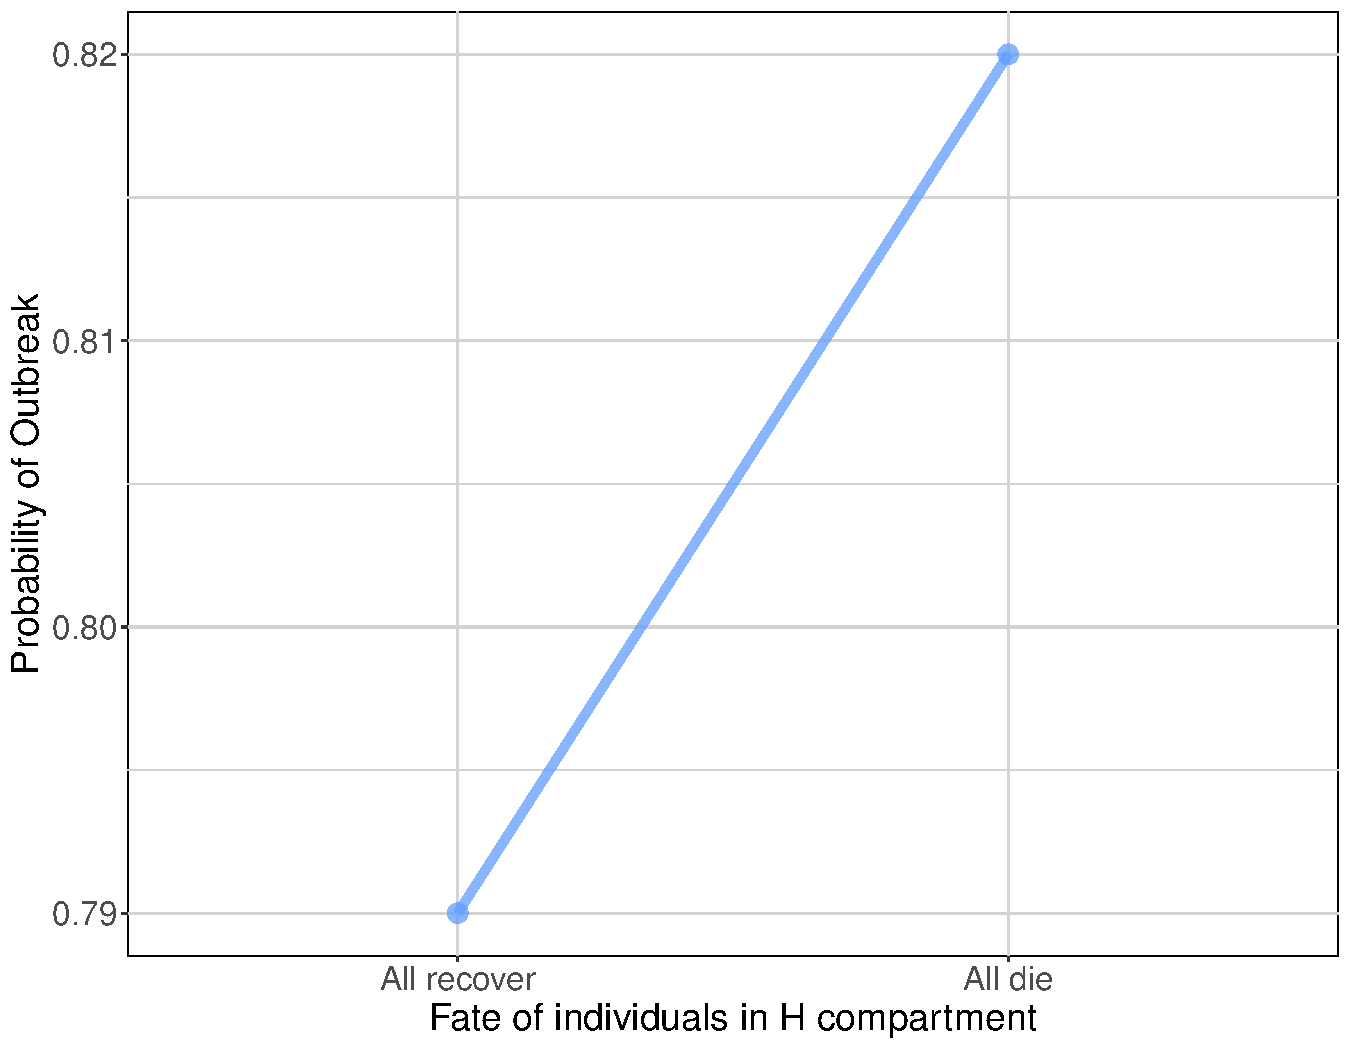
\includegraphics[width=0.31\textwidth]{figures/FigS2a}\hspace{2mm}\includegraphics[width=0.31\textwidth]{figures/FigS2b}\hspace{2mm}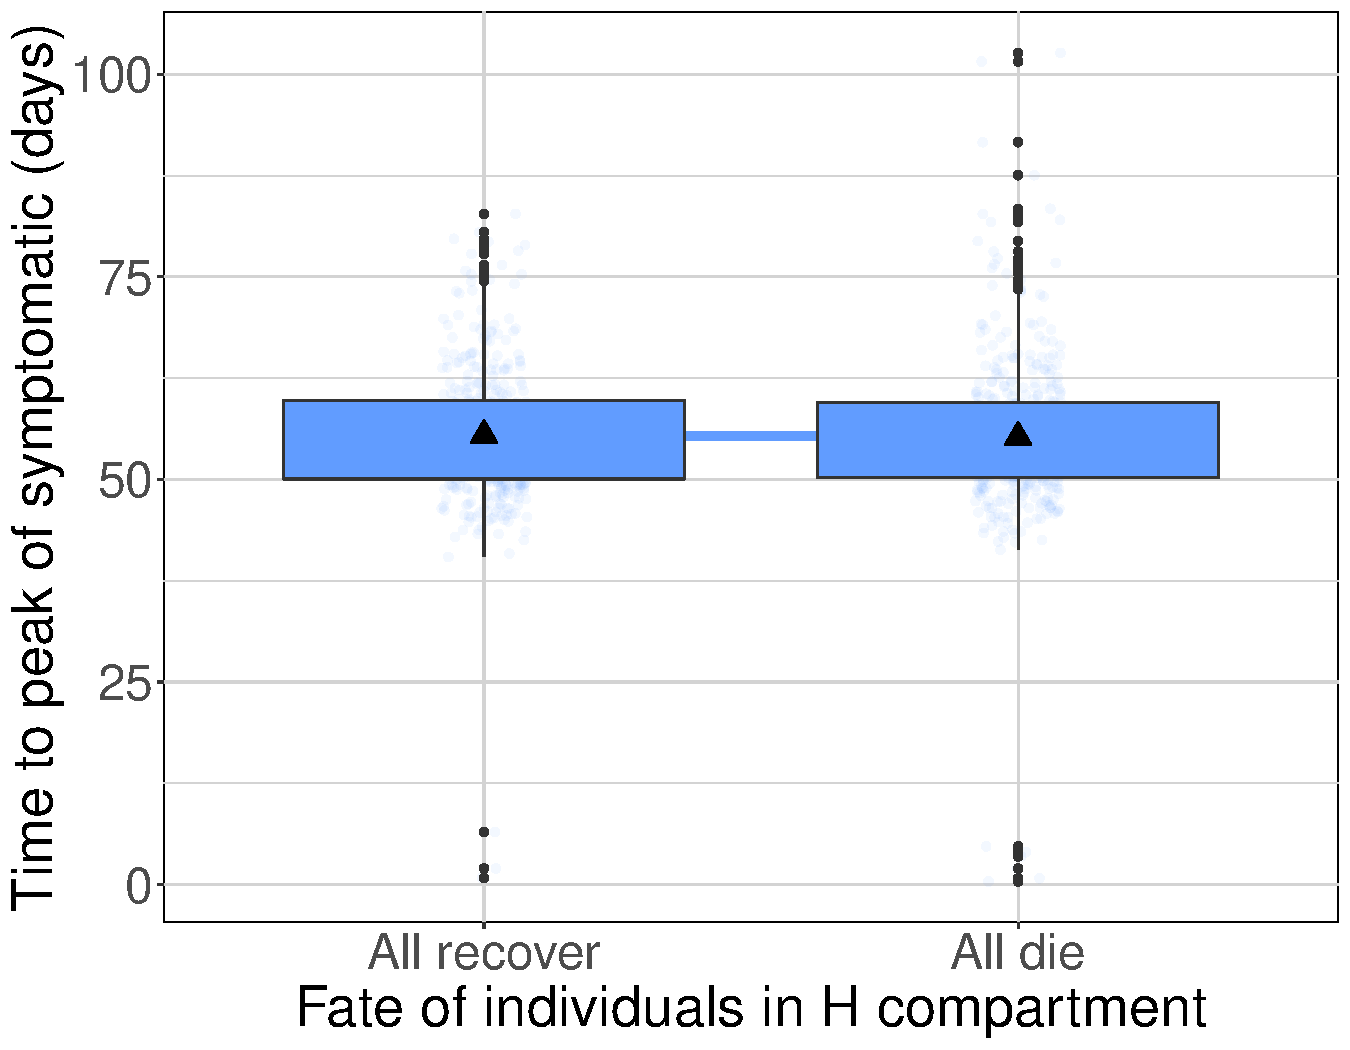
\includegraphics[width=0.31\textwidth]{figures/FigS2c}\\\medskip{}
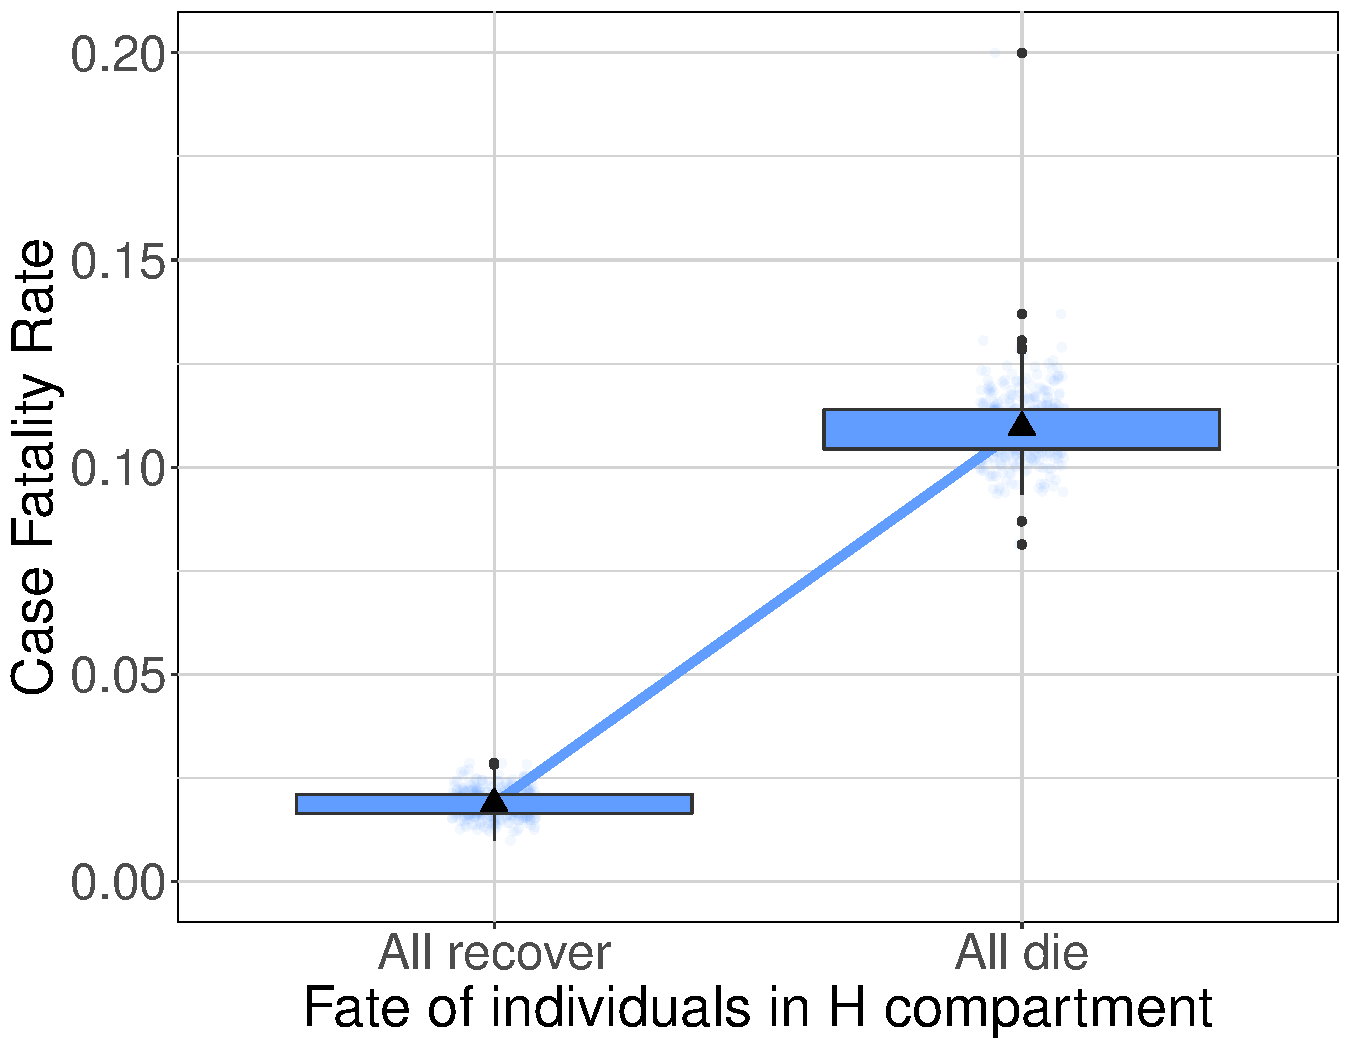
\includegraphics[width=0.31\textwidth]{figures/FigS2d}\hspace{2mm}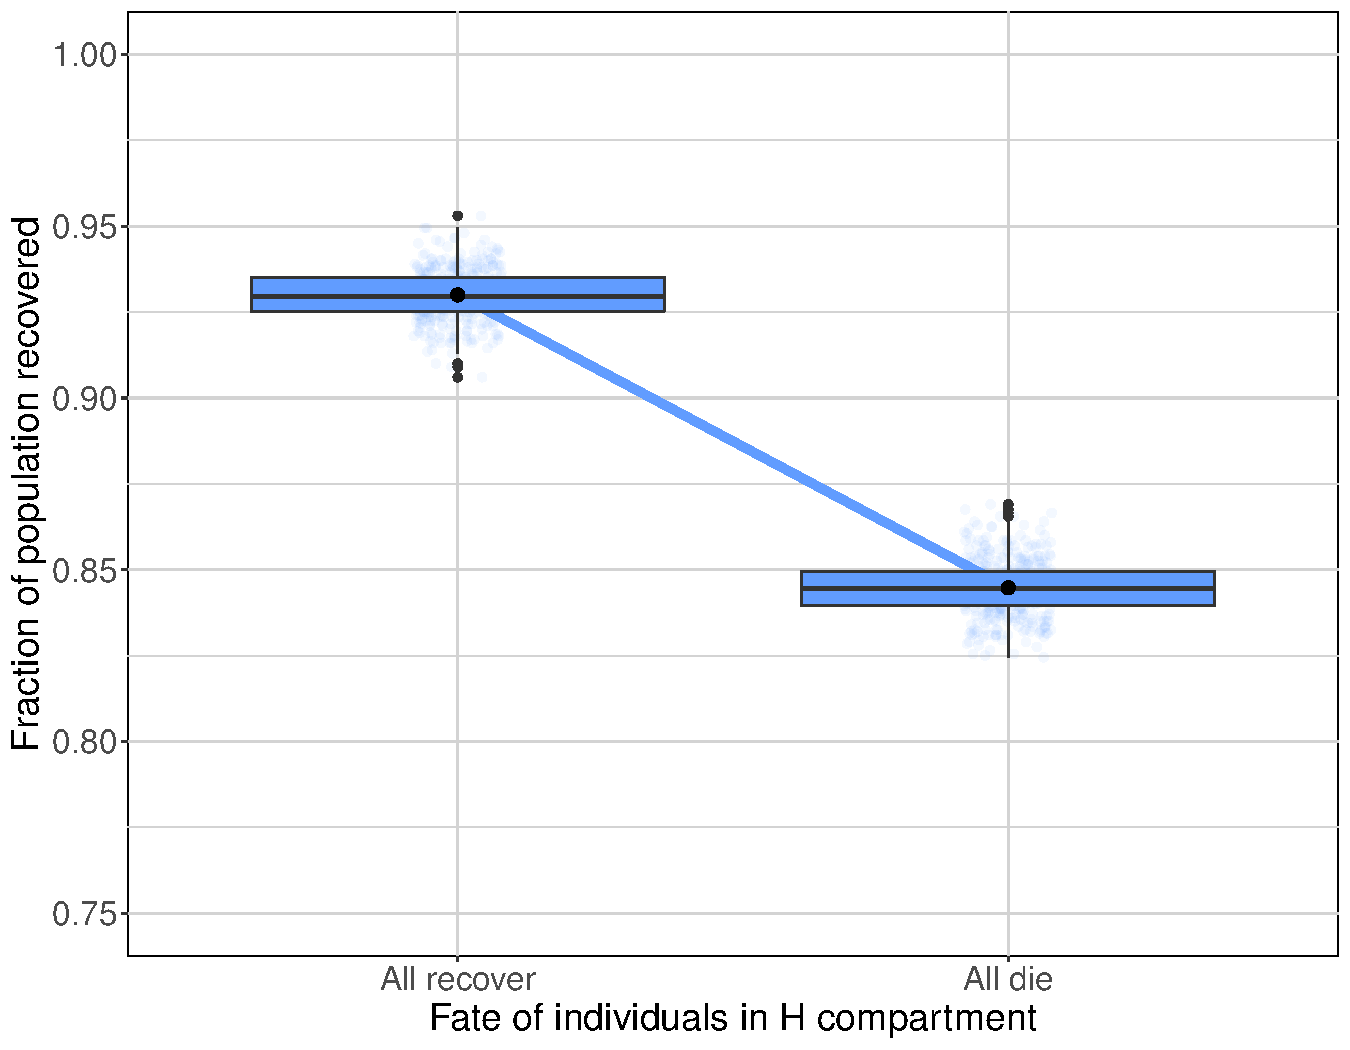
\includegraphics[width=0.31\textwidth]{figures/FigS2e}\caption{\label{fig:Suppl_DvsR} \textbf{Lower and upper bounds when interventions
are absent.} Probability of outbreak (top-left), fraction of casualties
(top-middle), time in which the number of symptomatic cases peaks
(top-right), CFR (bottom-left) and fraction of recovered individuals
(bottom-right), as a function of the fate of the individuals in the
H compartment, that may all recover or all die.}
\par\end{centering}
\end{figure}

\medskip{}

\begin{figure}[H]
\centering{}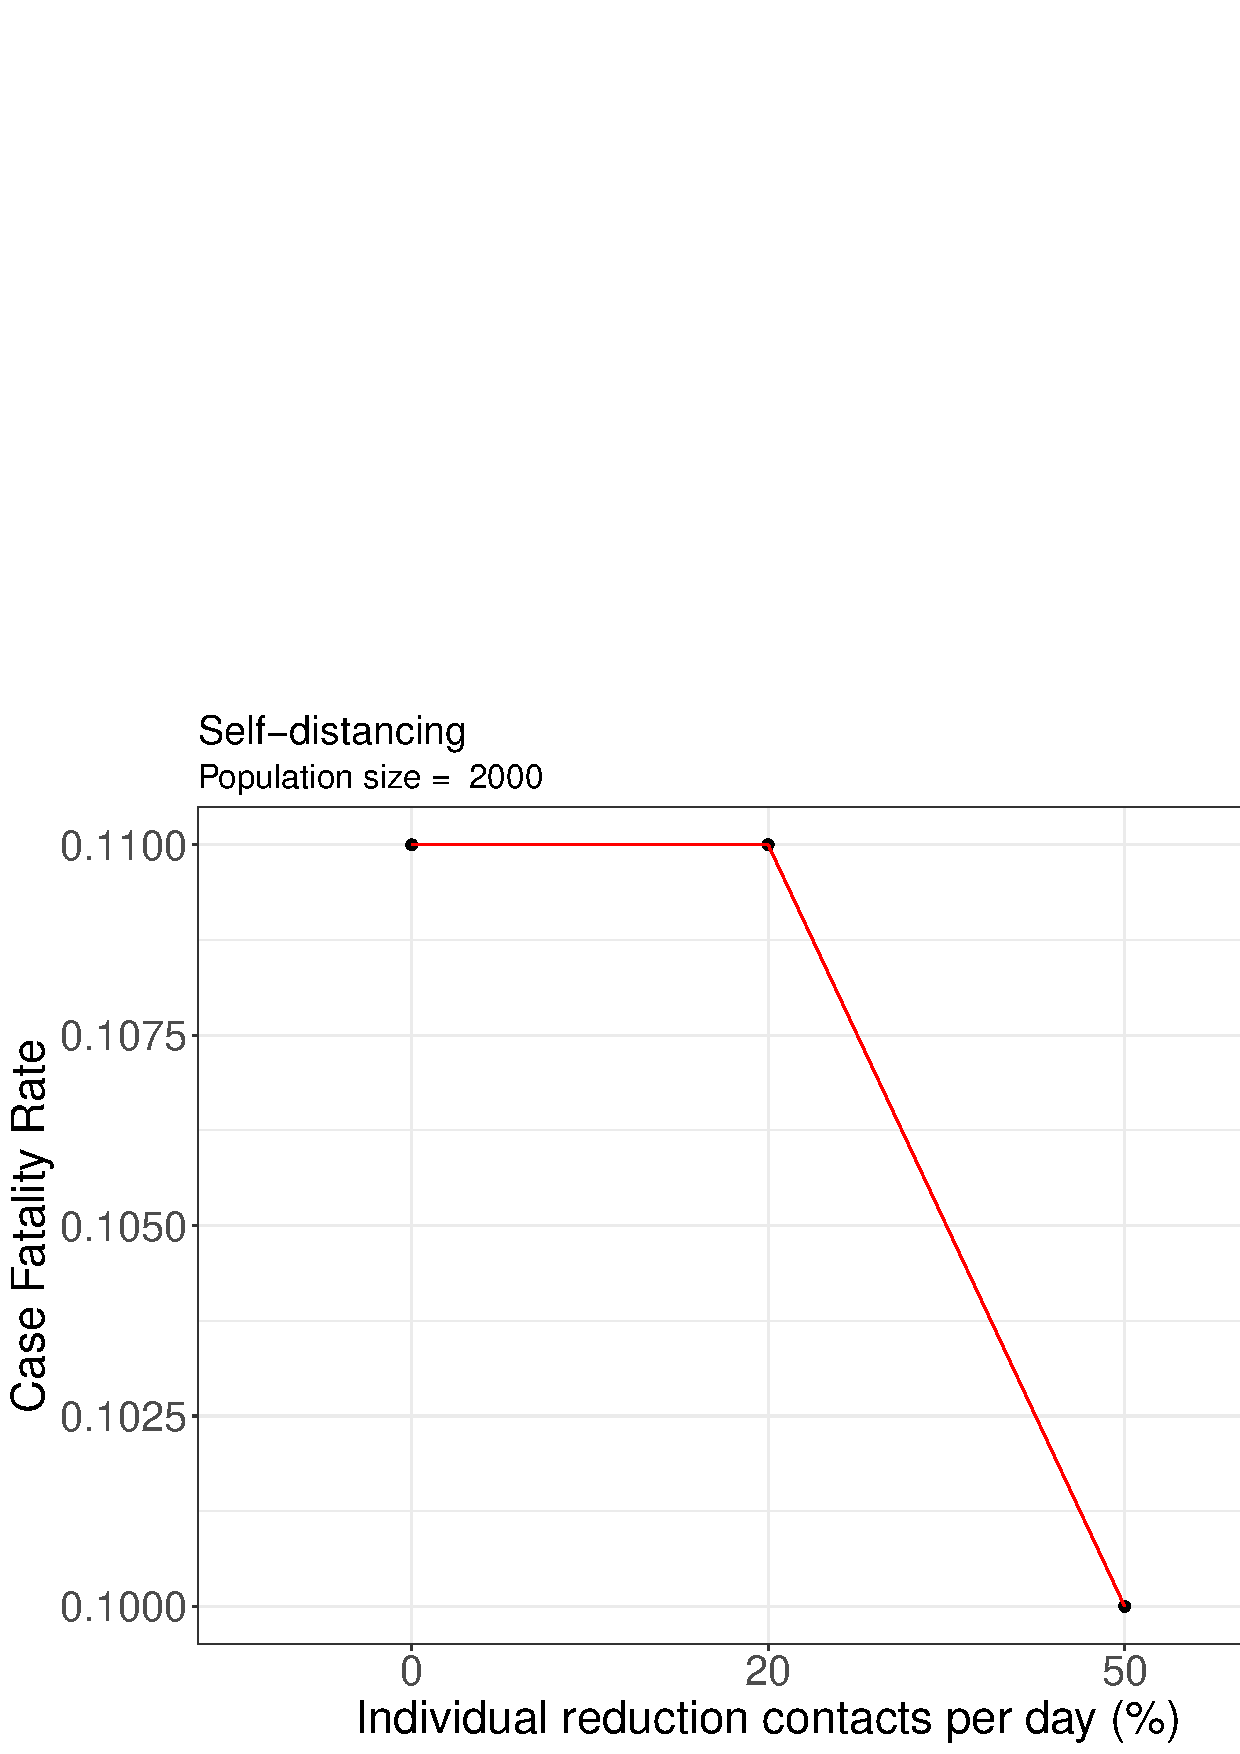
\includegraphics[width=0.31\textwidth]{figures/FigS3a}\hspace{2mm}\includegraphics[width=0.31\textwidth]{figures/FigS3b}\caption{\label{fig:Suppl_self} \textbf{Self-distancing.} CFR (left), and
fraction of recovered population (right) as a function of the reduction
in the fraction of contacts that the whole population experience self-distancing.}
\end{figure}
\medskip{}

\begin{figure}[H]
\centering{}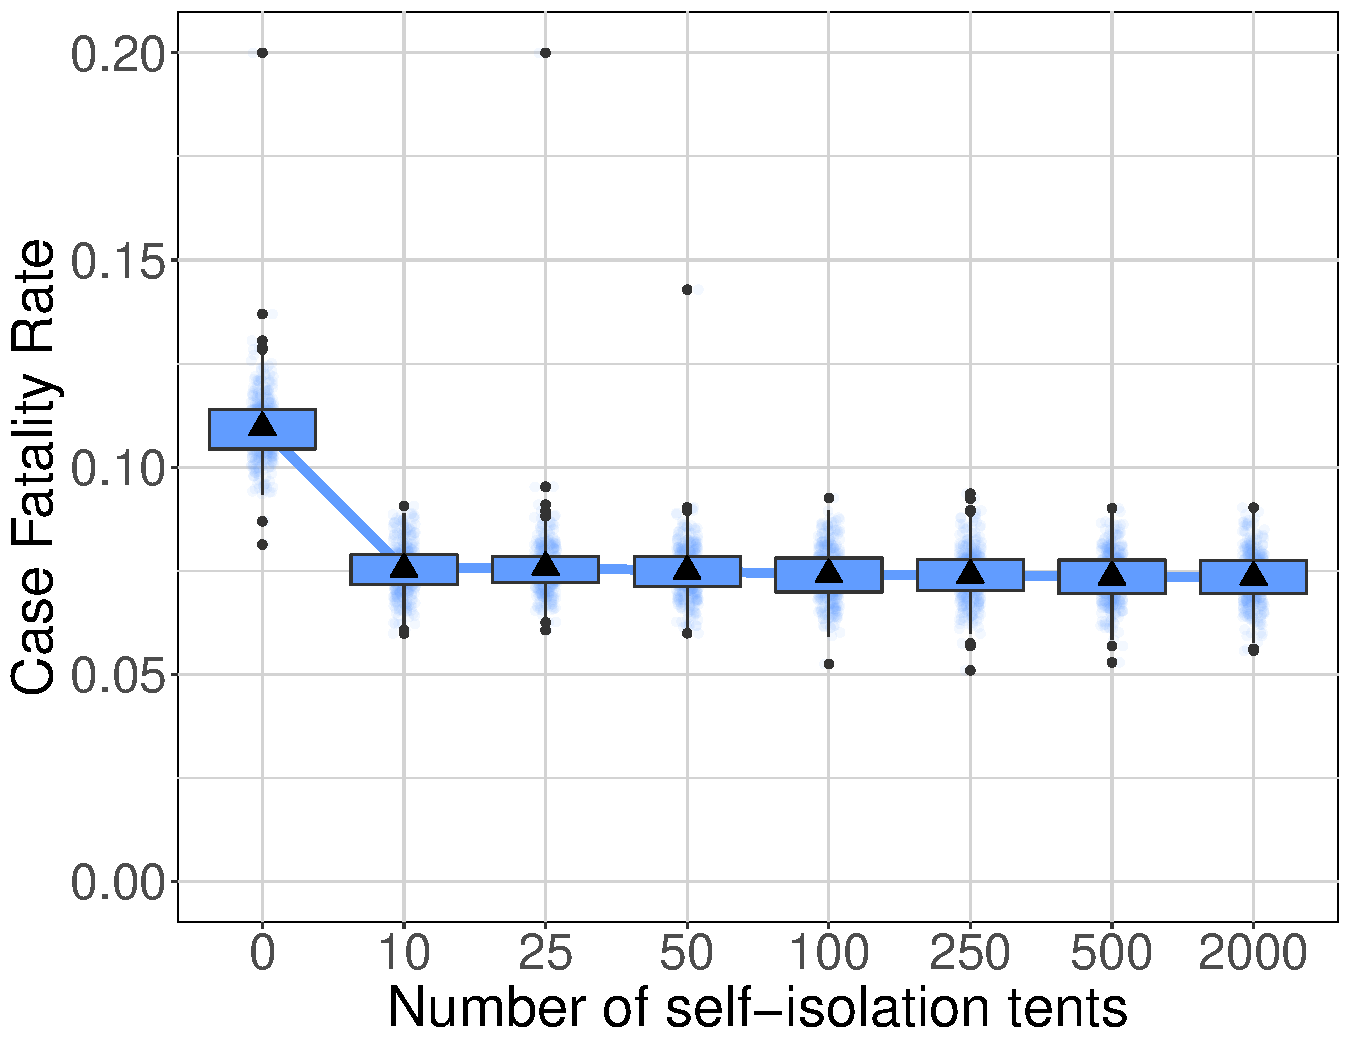
\includegraphics[width=0.31\textwidth]{figures/FigS4a}\hspace{2mm}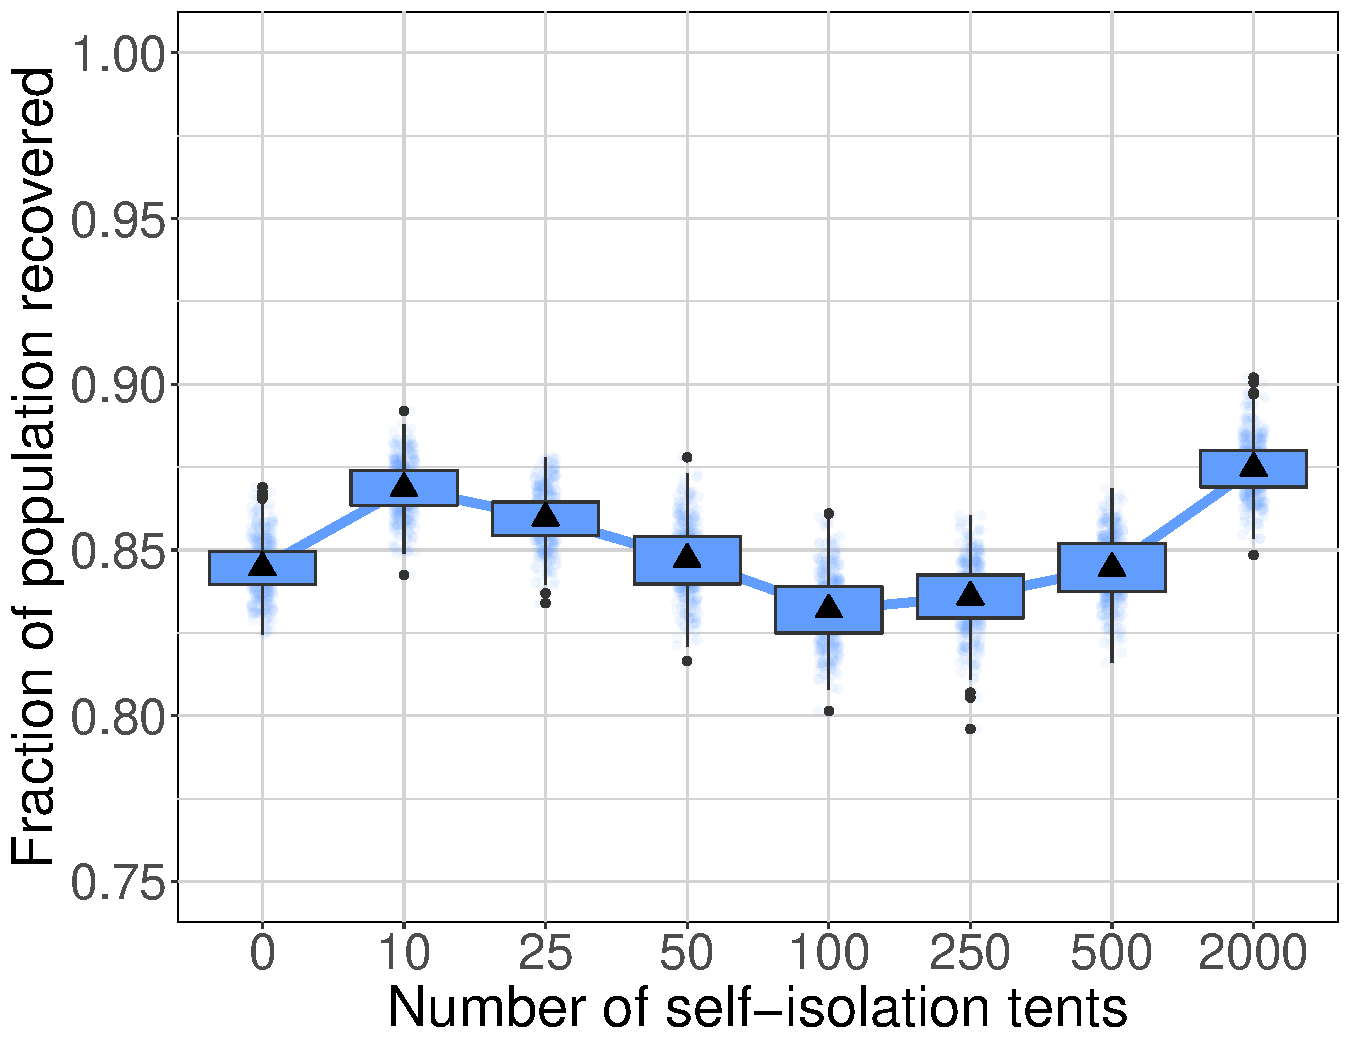
\includegraphics[width=0.31\textwidth]{figures/FigS4b}\caption{\label{fig:Suppl_isolation} \textbf{Self-isolation.} CFR (left),
and fraction of recovered population (right) as a function of the
number of tents available in the camp.}
\end{figure}

\medskip{}

\begin{figure}[H]
\centering{}\includegraphics[width=0.31\textwidth]{figures/FigS5a}\hspace{2mm}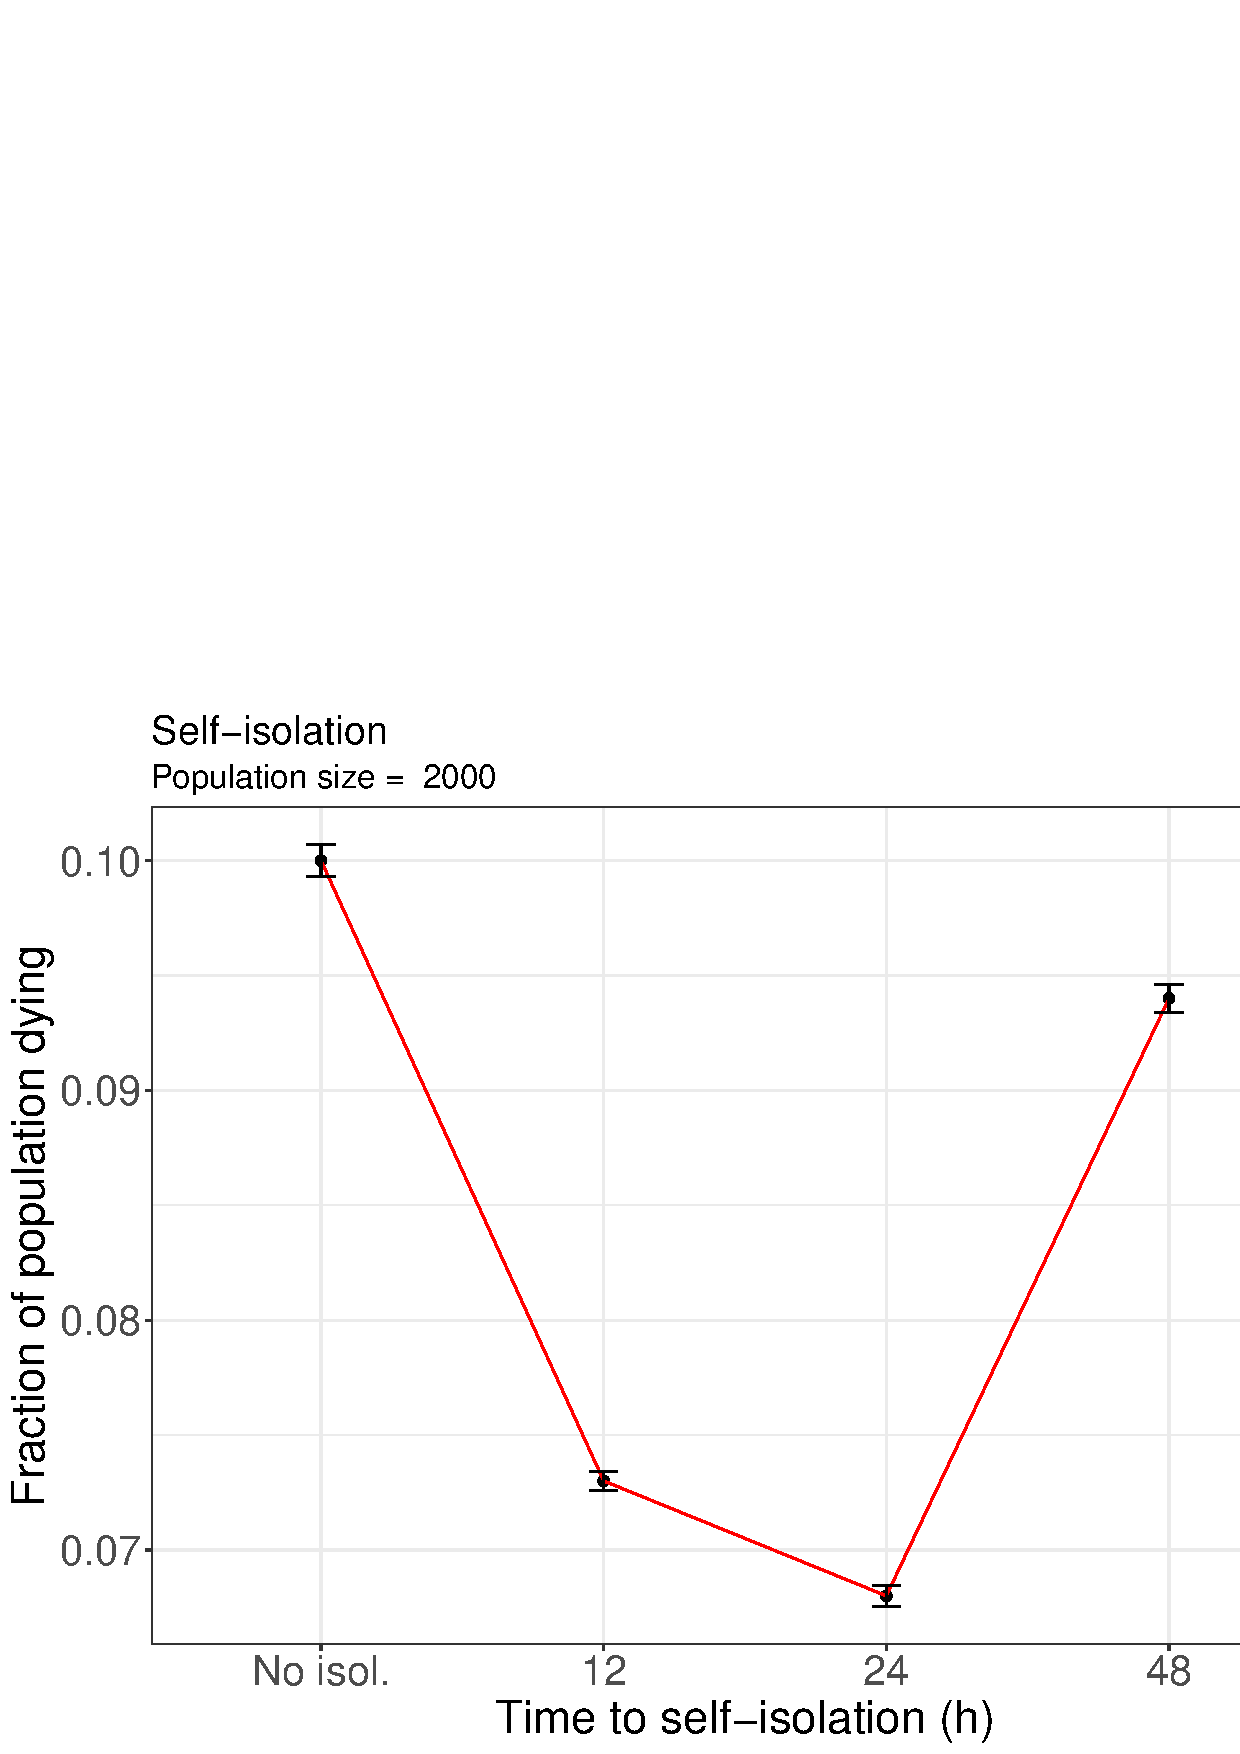
\includegraphics[width=0.31\textwidth]{figures/FigS5b}\hspace{2mm}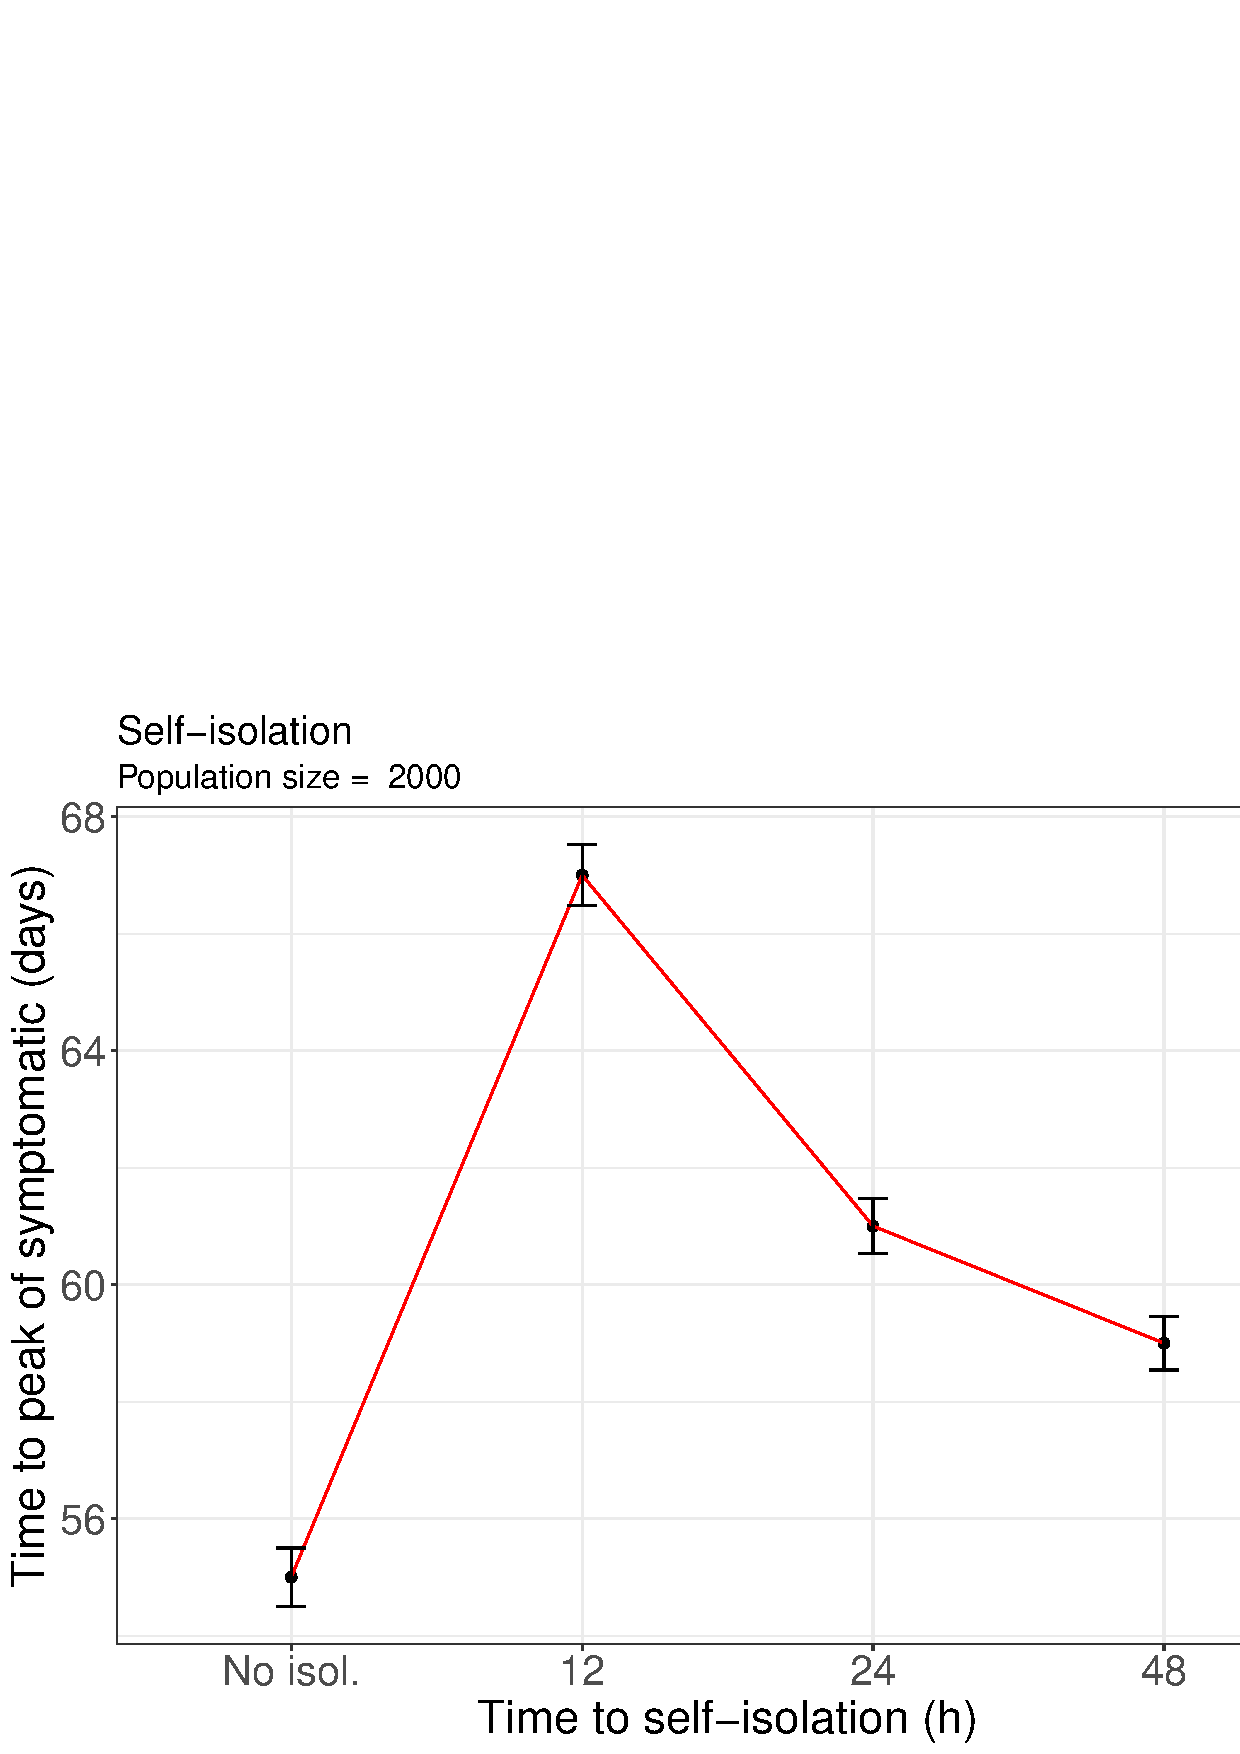
\includegraphics[width=0.31\textwidth]{figures/FigS5c}\\\medskip{}
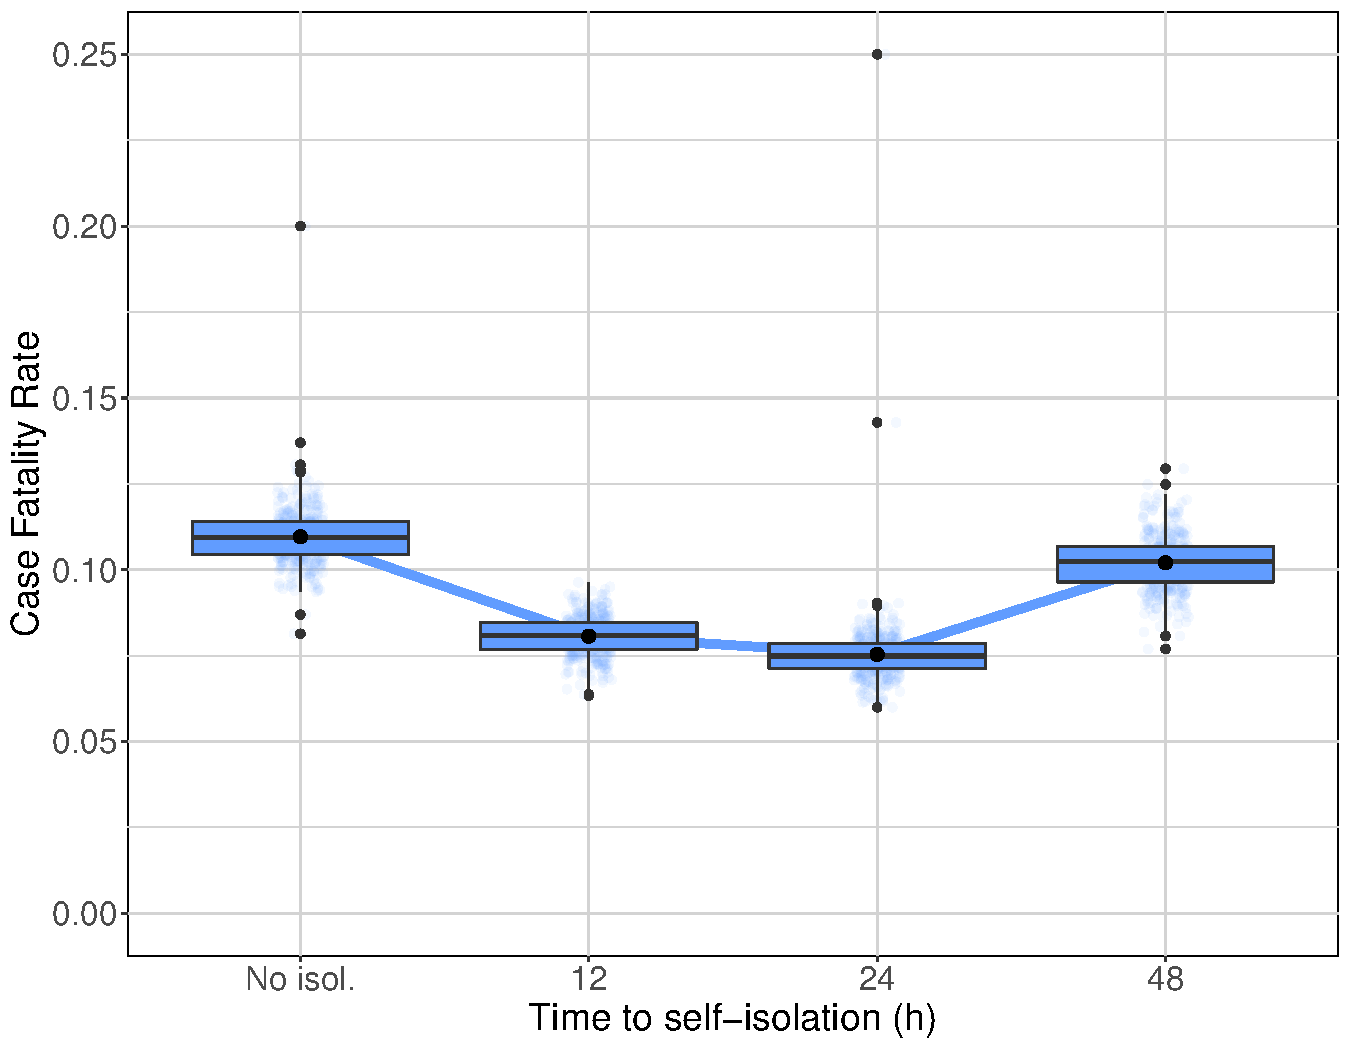
\includegraphics[width=0.31\textwidth]{figures/FigS5d}\hspace{2mm}\includegraphics[width=0.31\textwidth]{figures/FigS5e}\caption{\label{fig:Suppl_onset} \textbf{Time to self-isolation.} Probability
of outbreak (top-left), fraction of casualties (top-middle), time
in which the number of symptomatic cases peaks (top-right), CFR (bottom-left)
and fraction of recovered individuals (bottom-right), as a function
of the time that individuals require to recognize their symptoms and
self-isolate.}
\end{figure}

\medskip{}

\begin{figure}[H]
\centering{}\includegraphics[width=0.31\textwidth]{figures/FigS6a}\hspace{2mm}\includegraphics[width=0.31\textwidth]{figures/FigS6b}\hspace{2mm}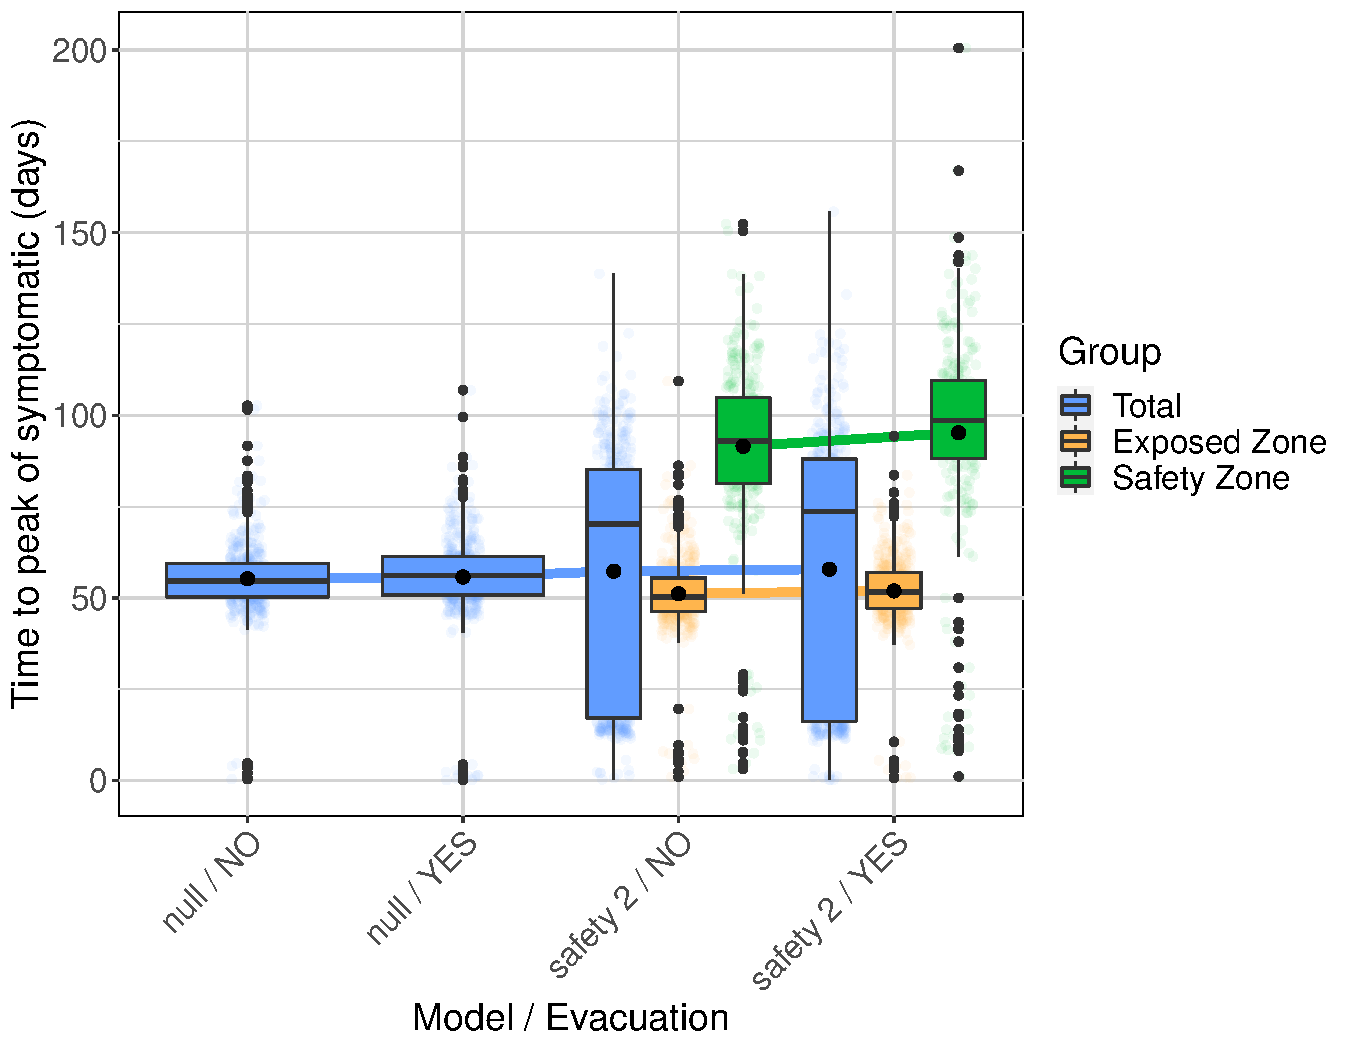
\includegraphics[width=0.31\textwidth]{figures/FigS6c}\\\medskip{}
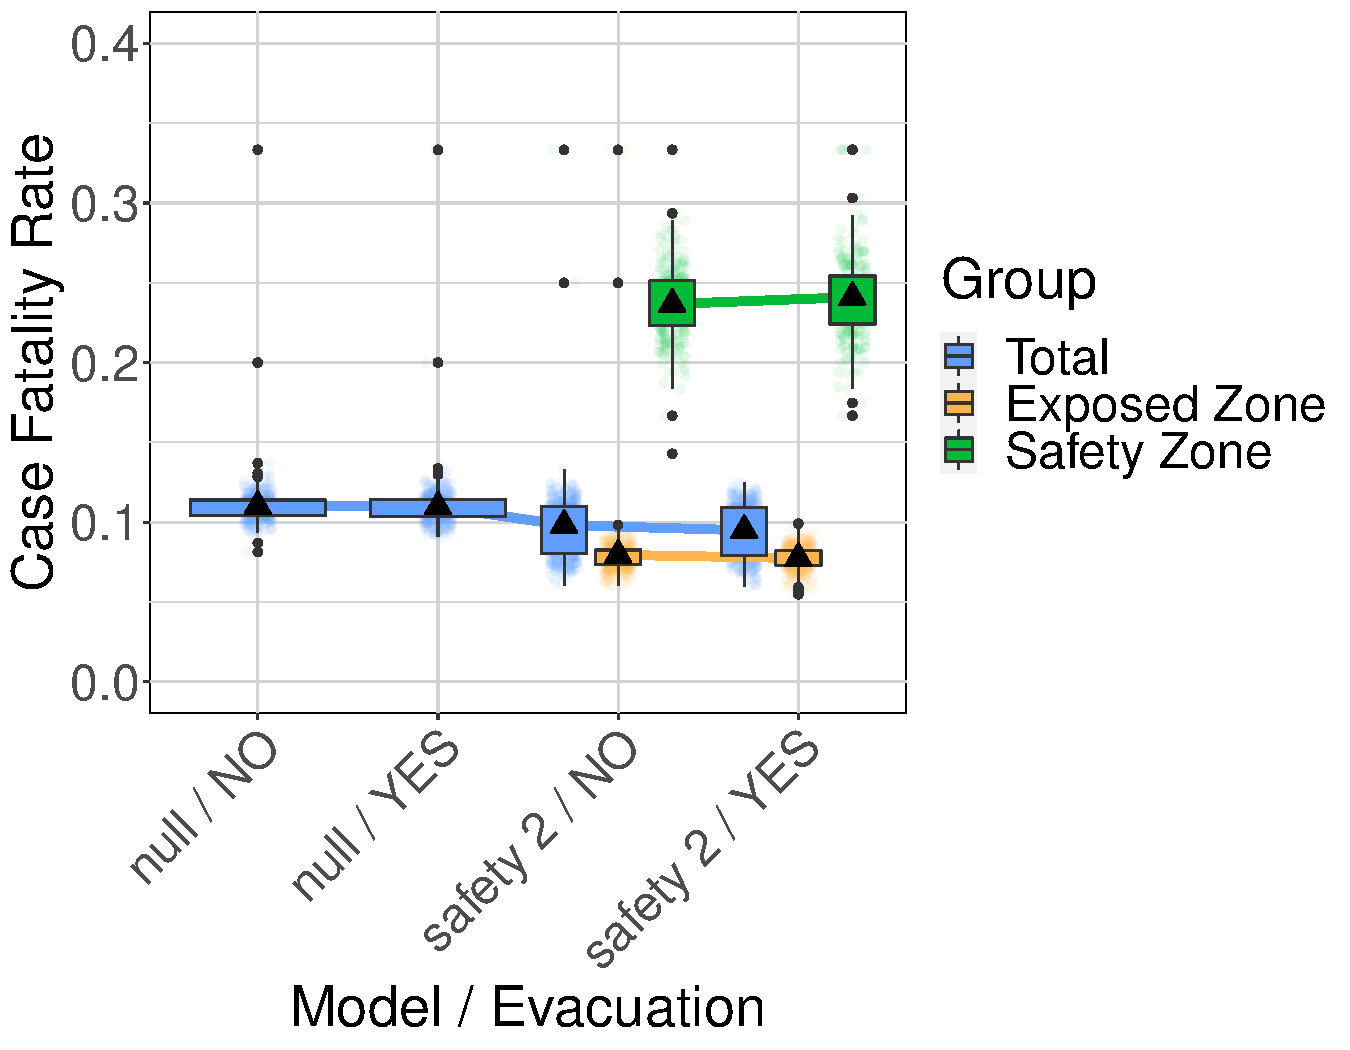
\includegraphics[width=0.31\textwidth]{figures/FigS6d}\hspace{2mm}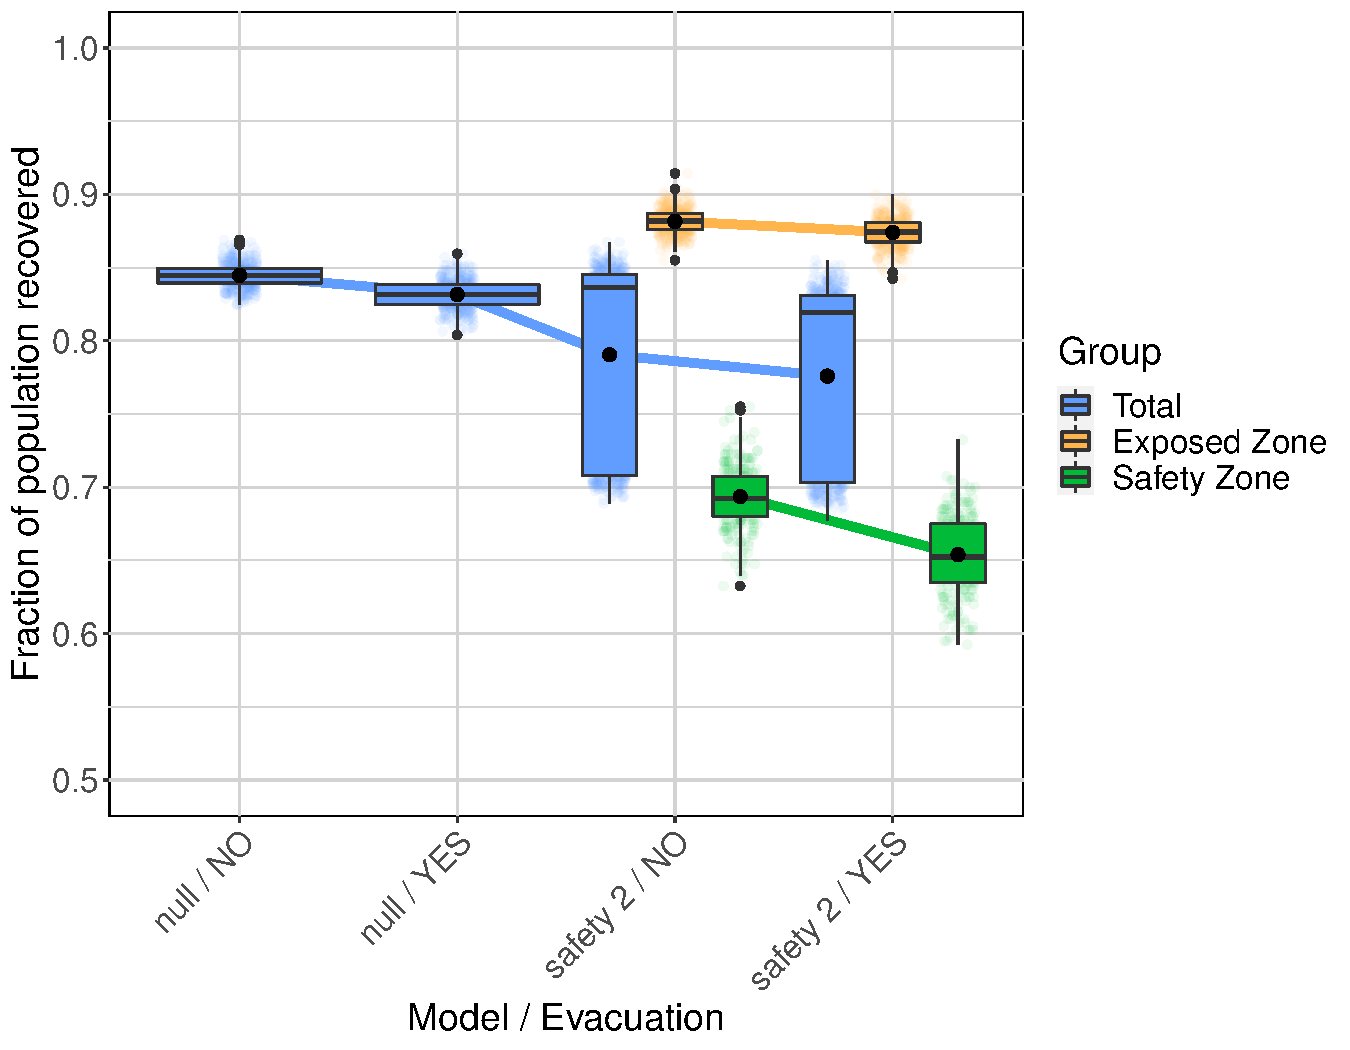
\includegraphics[width=0.31\textwidth]{figures/FigS6e}\caption{\label{fig:Suppl_evacuation} \textbf{Evacuation.} Probability of
outbreak (top-left), fraction of casualties (top-middle), time in
which the number of symptomatic cases peaks (top-right), CFR (bottom-left)
and fraction of recovered individuals (bottom-right), depending on
whether individuals requiring hospitalization are evacuated to isolation
centers.}
\end{figure}

\medskip{}

\begin{figure}[H]
\begin{centering}
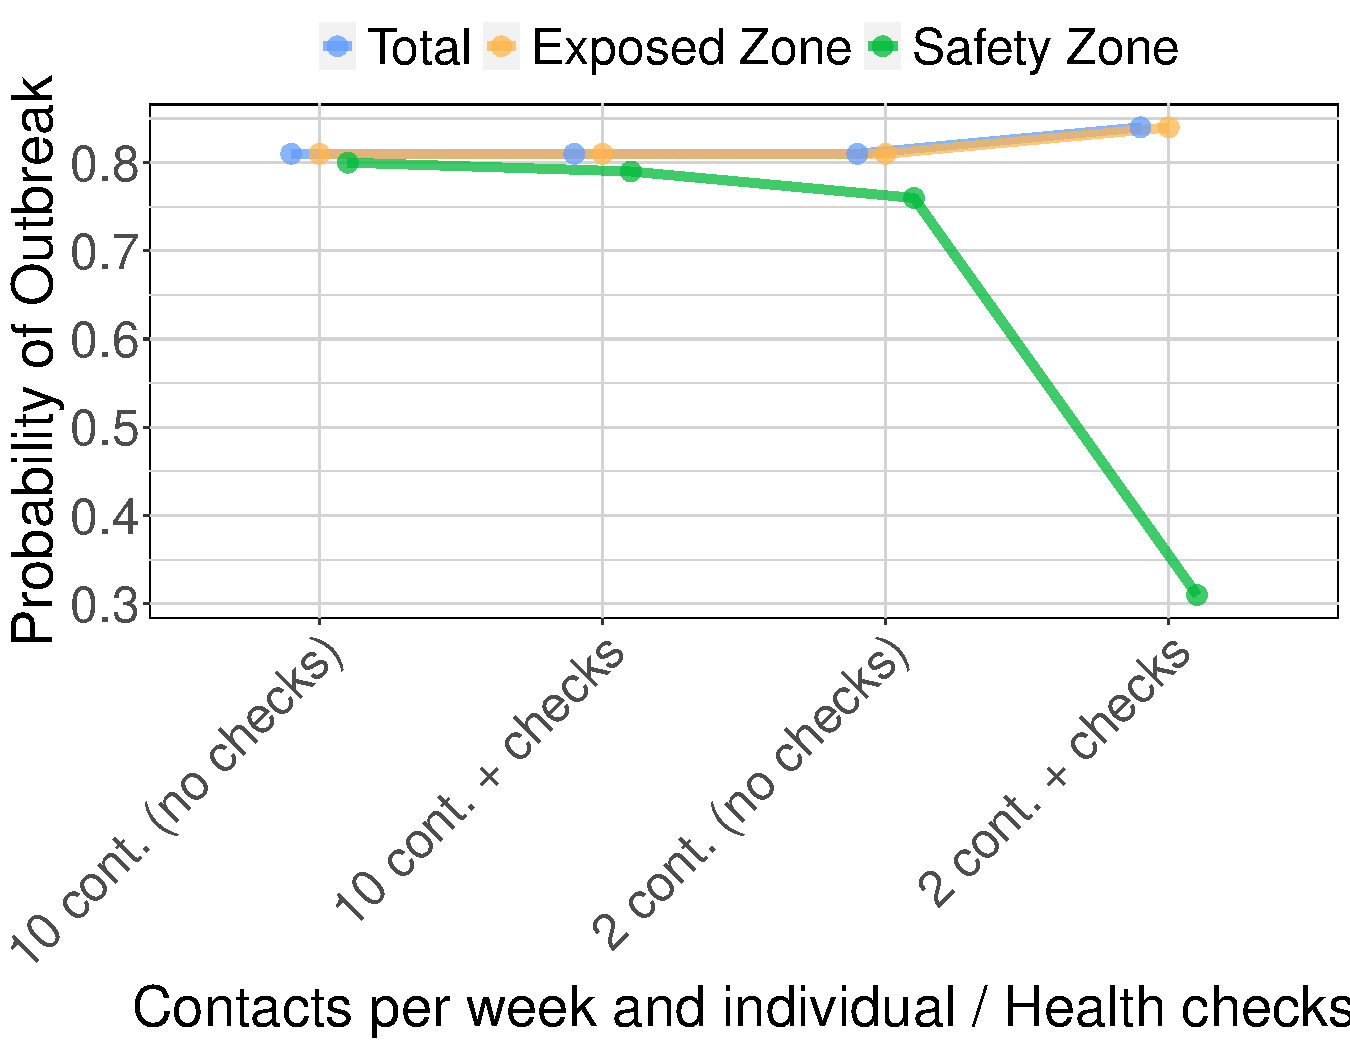
\includegraphics[width=0.31\textwidth]{figures/FigS7a}\hspace{2mm}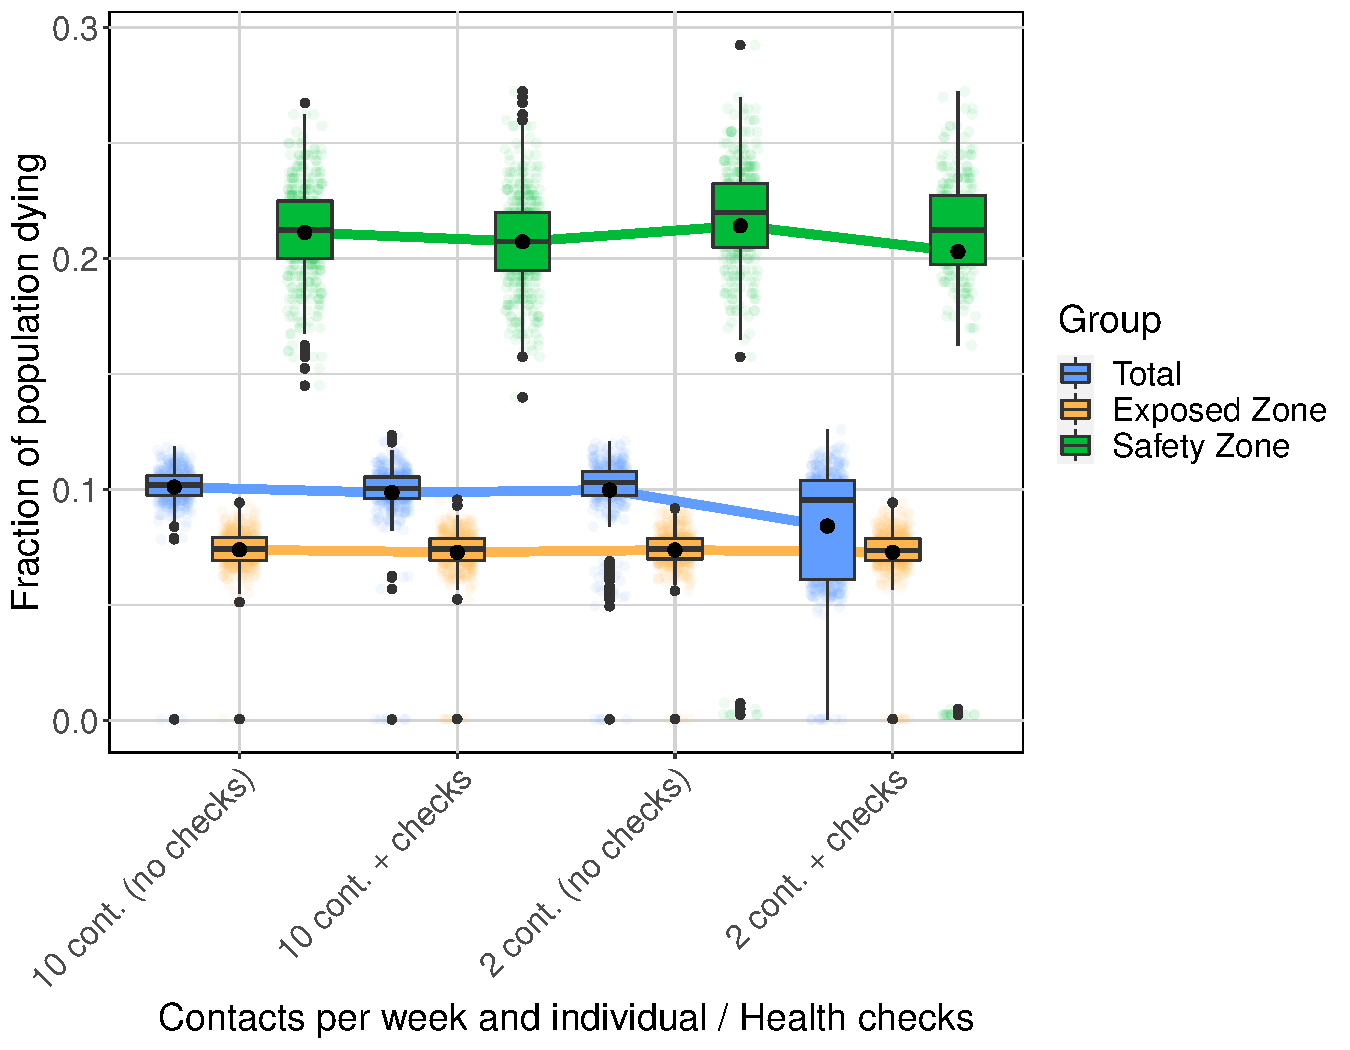
\includegraphics[width=0.31\textwidth]{figures/FigS7b}\hspace{2mm}\includegraphics[width=0.31\textwidth]{figures/FigS7c}\\\medskip{}
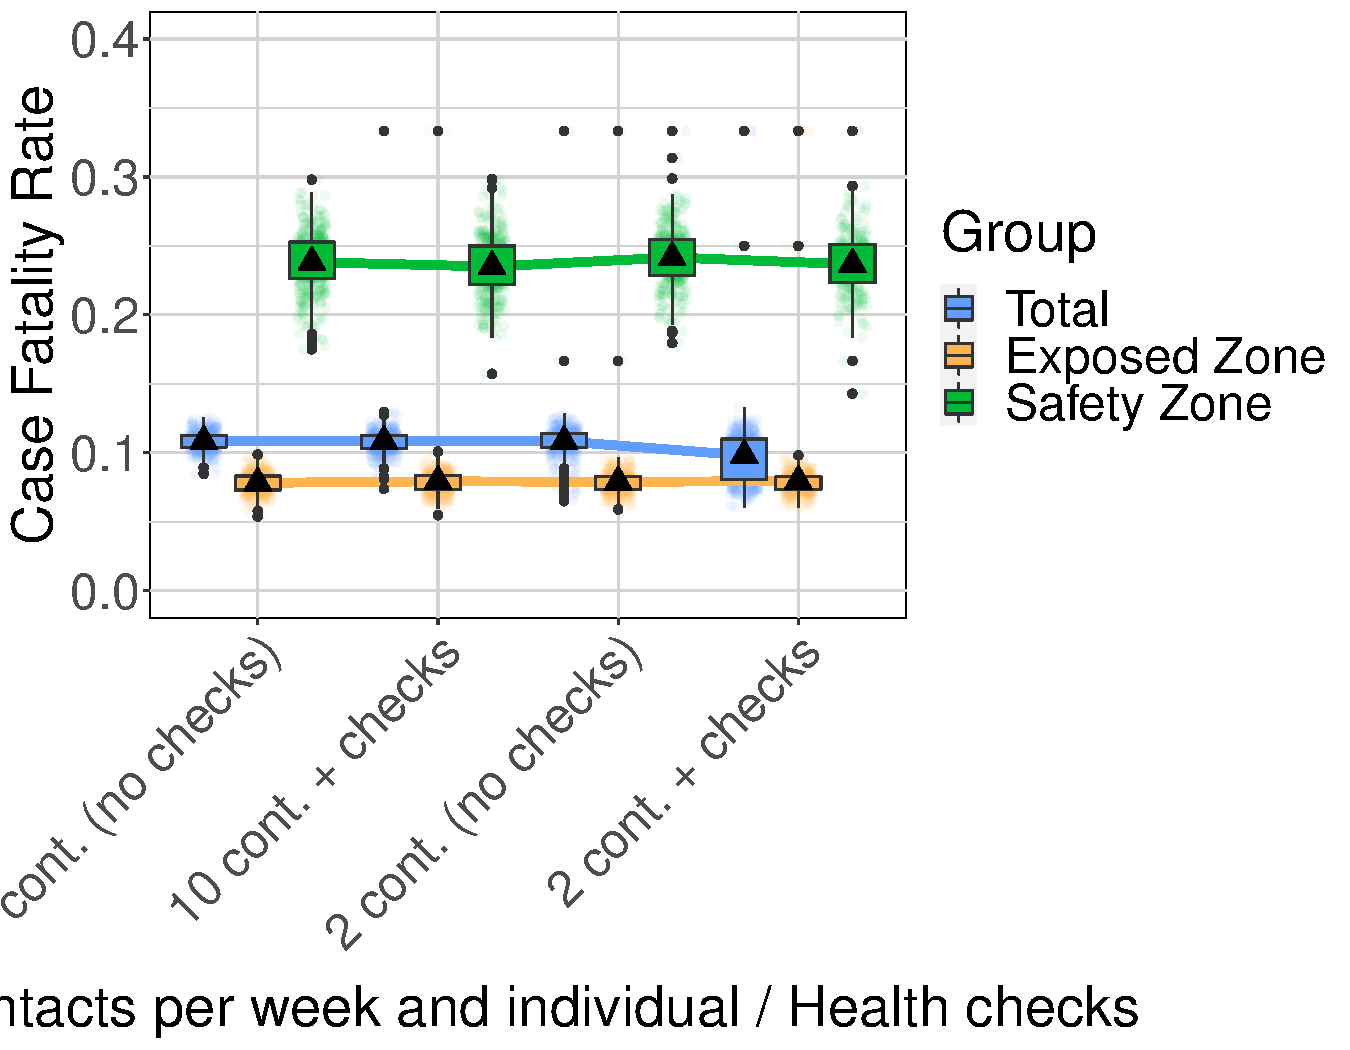
\includegraphics[width=0.31\textwidth]{figures/FigS7d}\hspace{2mm}\includegraphics[width=0.31\textwidth]{figures/FigS7e}
\par\end{centering}
\caption{\label{fig:Suppl_Tcheck} \textbf{Health-checks in the buffering zone.}
Probability of outbreak (top-left), fraction of casualties (top-middle),
time in which the number of symptomatic cases peaks (top-right), CFR
(bottom-left) and fraction of recovered individuals (bottom-right),
depending on whether health-checks are implemented to avoid that symptomatic
individuals access to the buffering zone separating the orange and
green zones.}
\end{figure}

\medskip{}

\begin{figure}[H]
\centering{}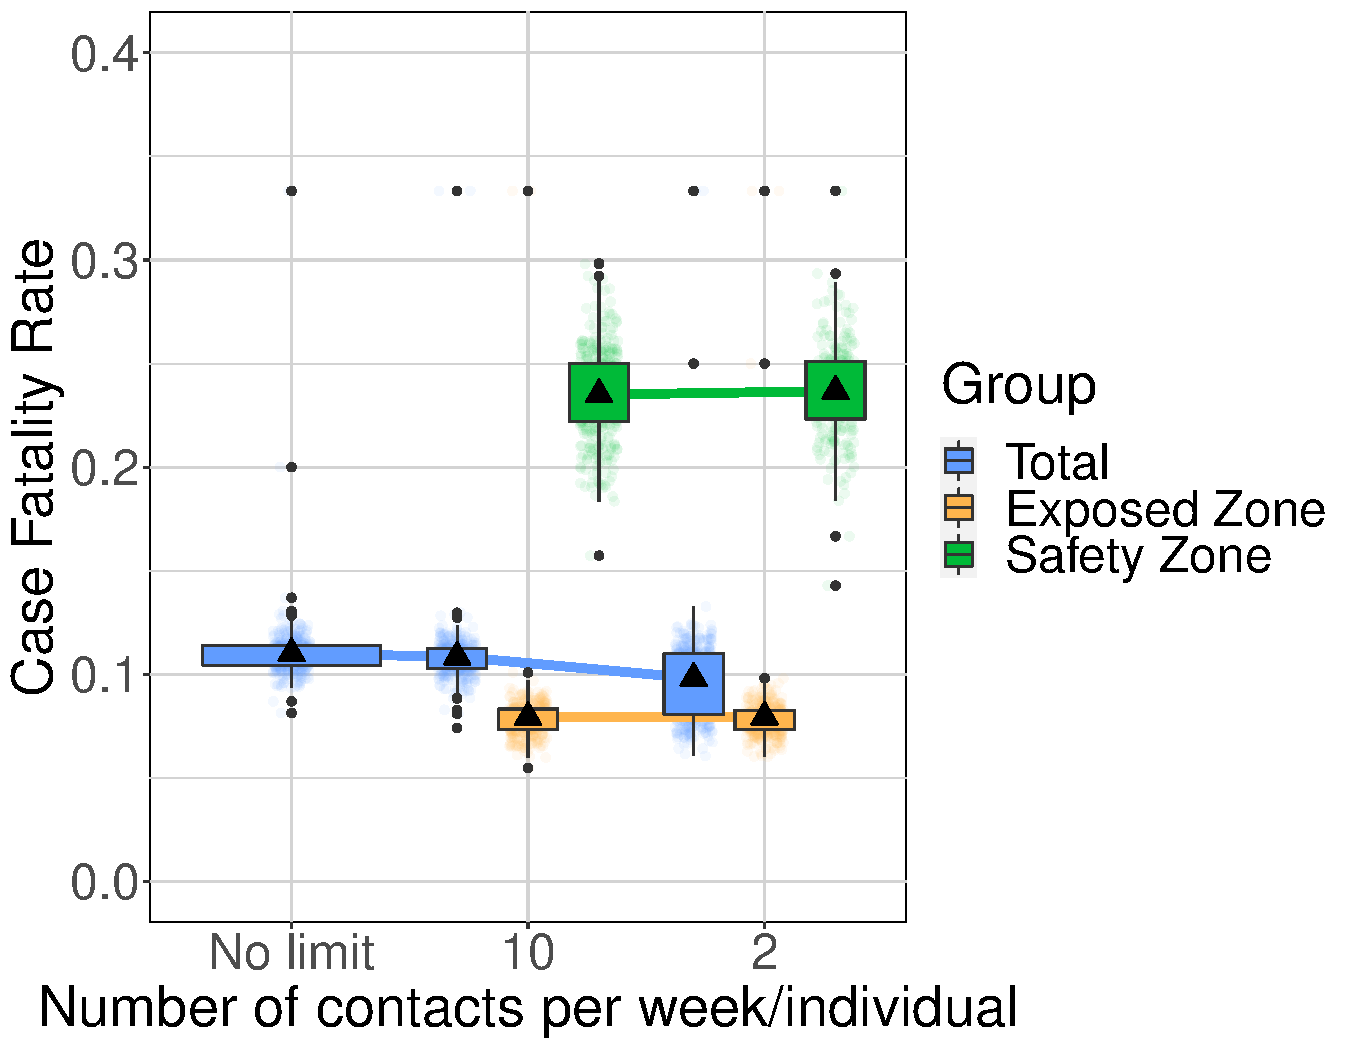
\includegraphics[width=0.31\textwidth]{figures/FigS8a}\hspace{2mm}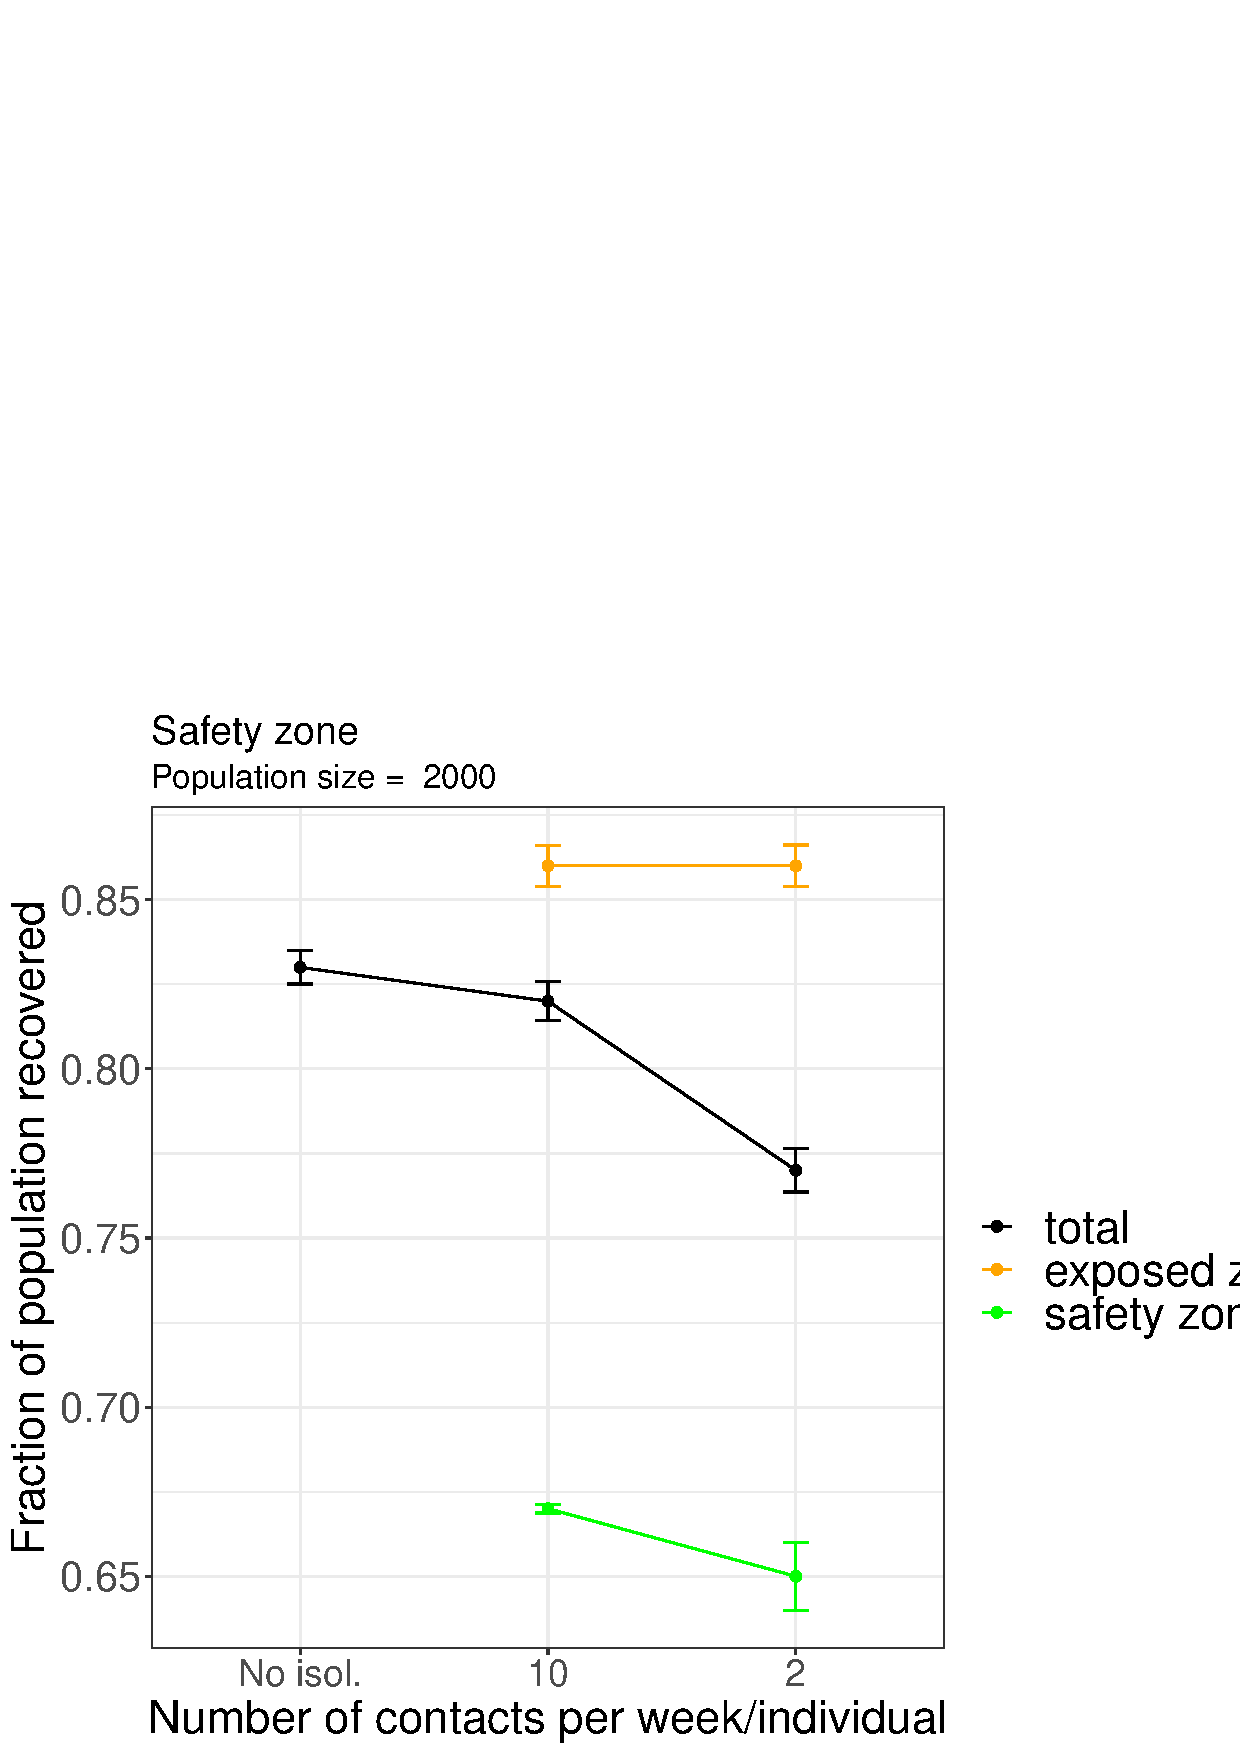
\includegraphics[width=0.31\textwidth]{figures/FigS8b}\caption{\label{fig:Suppl_safety} \textbf{Number of contacts in the buffering
zone.} CFR (left), and fraction of recovered population (right) as
a function of the number of contacts per week and individual permitted
in the buffering zone, in which the populations living in the green
and orange zones are allowed to interact.}
\end{figure}
\medskip{}

\begin{figure}[H]
\begin{centering}
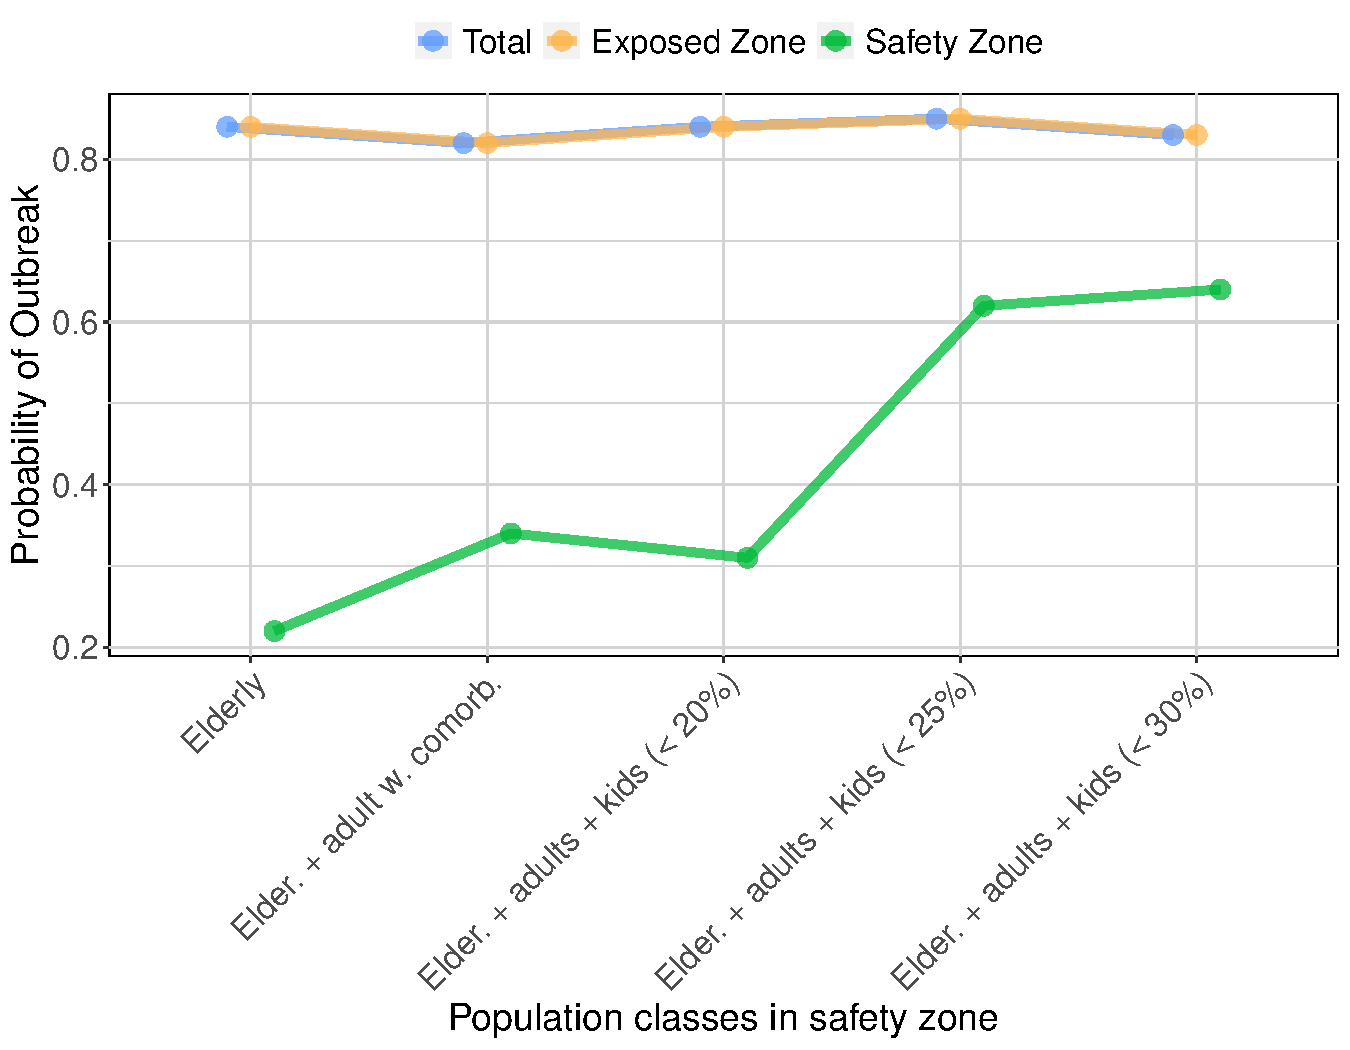
\includegraphics[width=0.31\textwidth]{figures/FigS9a}\hspace{2mm}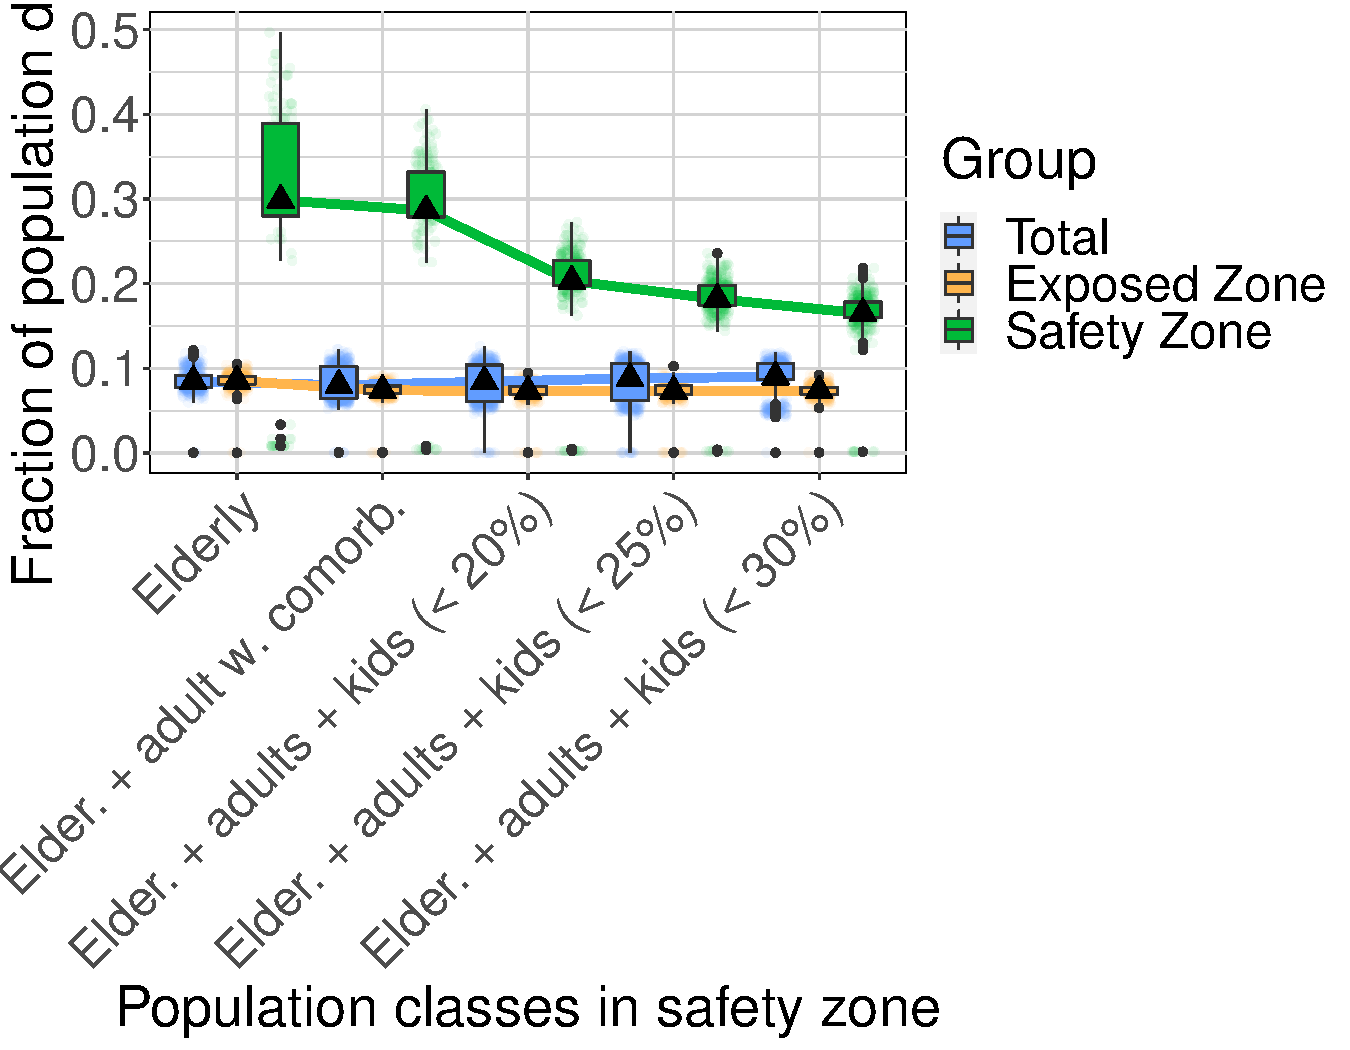
\includegraphics[width=0.31\textwidth]{figures/FigS9b}\hspace{2mm}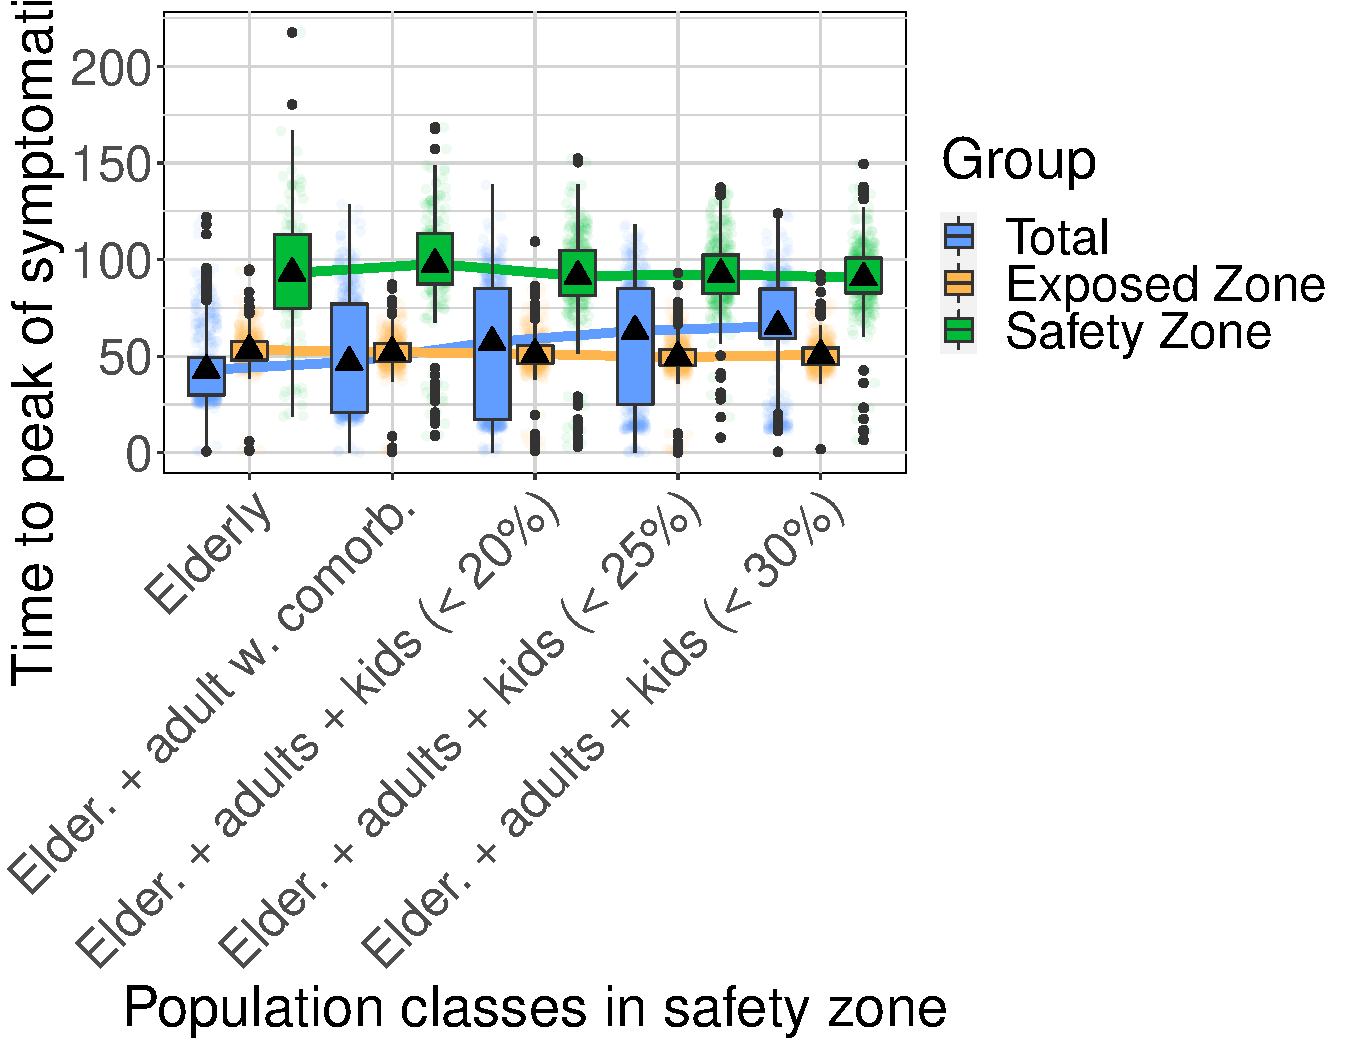
\includegraphics[width=0.31\textwidth]{figures/FigS9c}\\\medskip{}
\includegraphics[width=0.31\textwidth]{figures/FigS9d}\hspace{2mm}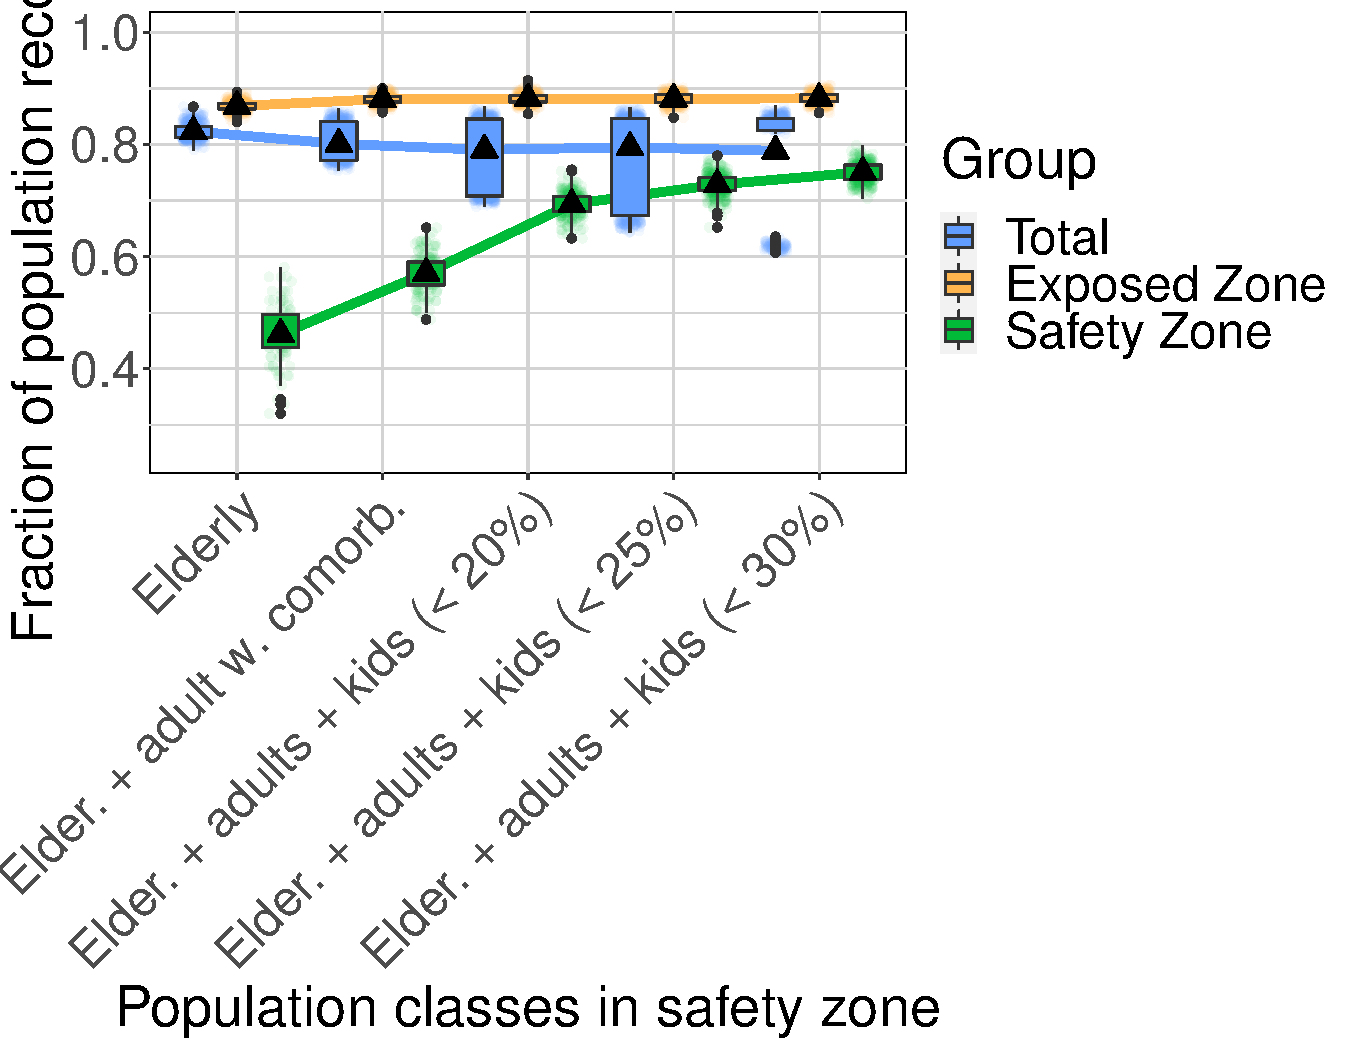
\includegraphics[width=0.31\textwidth]{figures/FigS9e}
\par\end{centering}
\caption{\label{fig:Suppl_popClass} \textbf{Population moving to the safety
zone.} Probability of outbreak (top-left), fraction of casualties
(top-middle), time in which the number of symptomatic cases peaks
(top-right), CFR (bottom-left) and fraction of recovered individuals
(bottom-right), as a function of the population moving to the safety
zone.}
\end{figure}
\medskip{}

\begin{figure}[H]
\begin{centering}
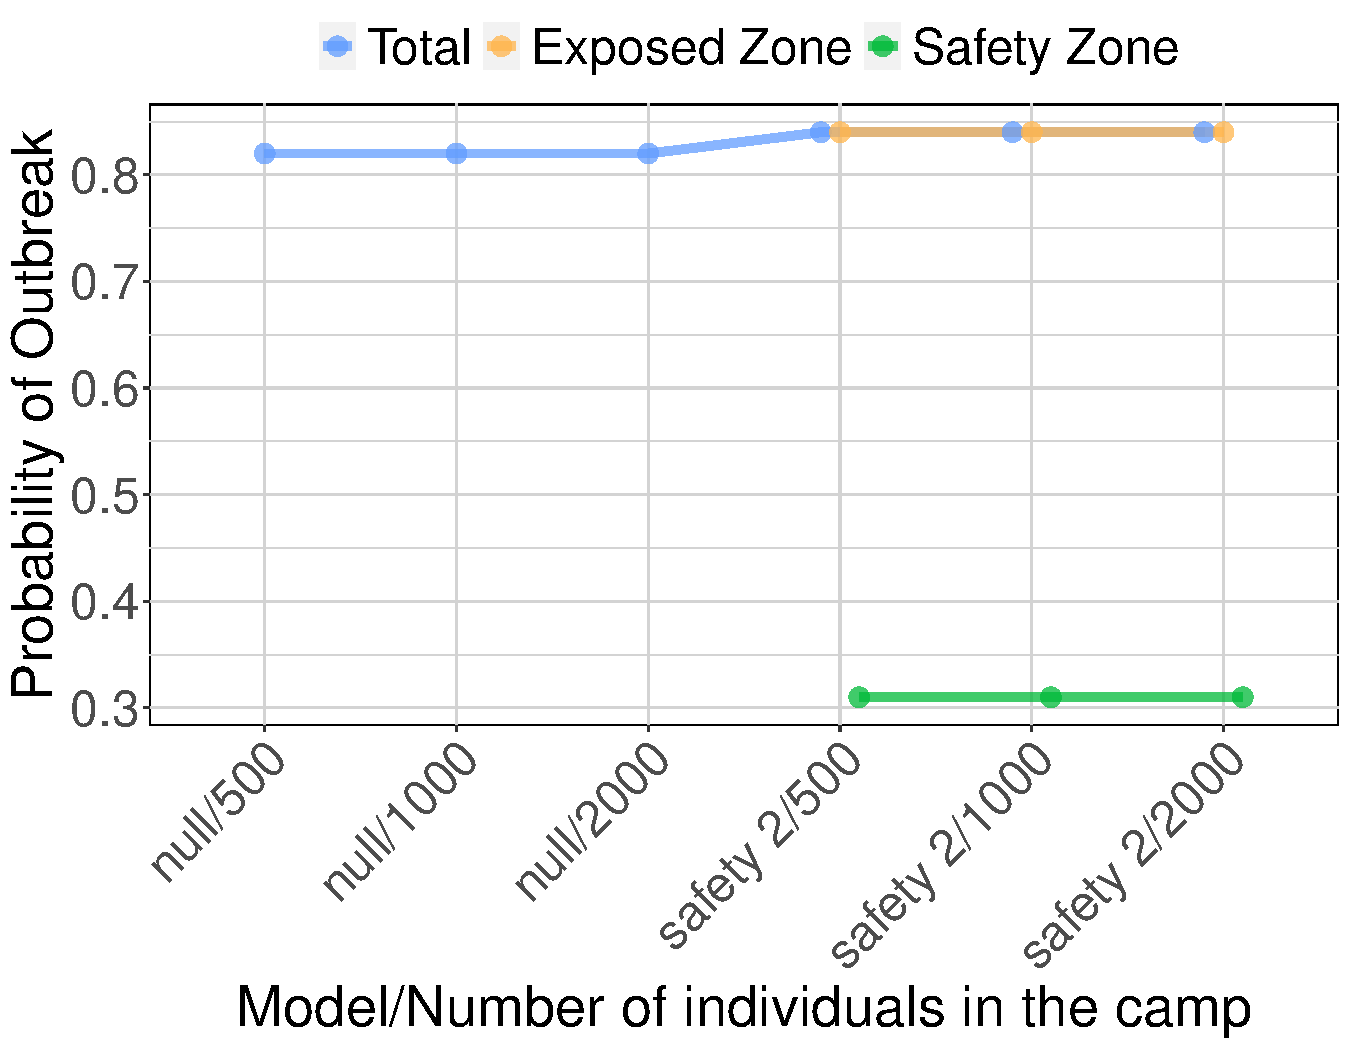
\includegraphics[width=0.31\textwidth]{figures/FigS10a}\hspace{2mm}\includegraphics[width=0.31\textwidth]{figures/FigS10b}\hspace{2mm}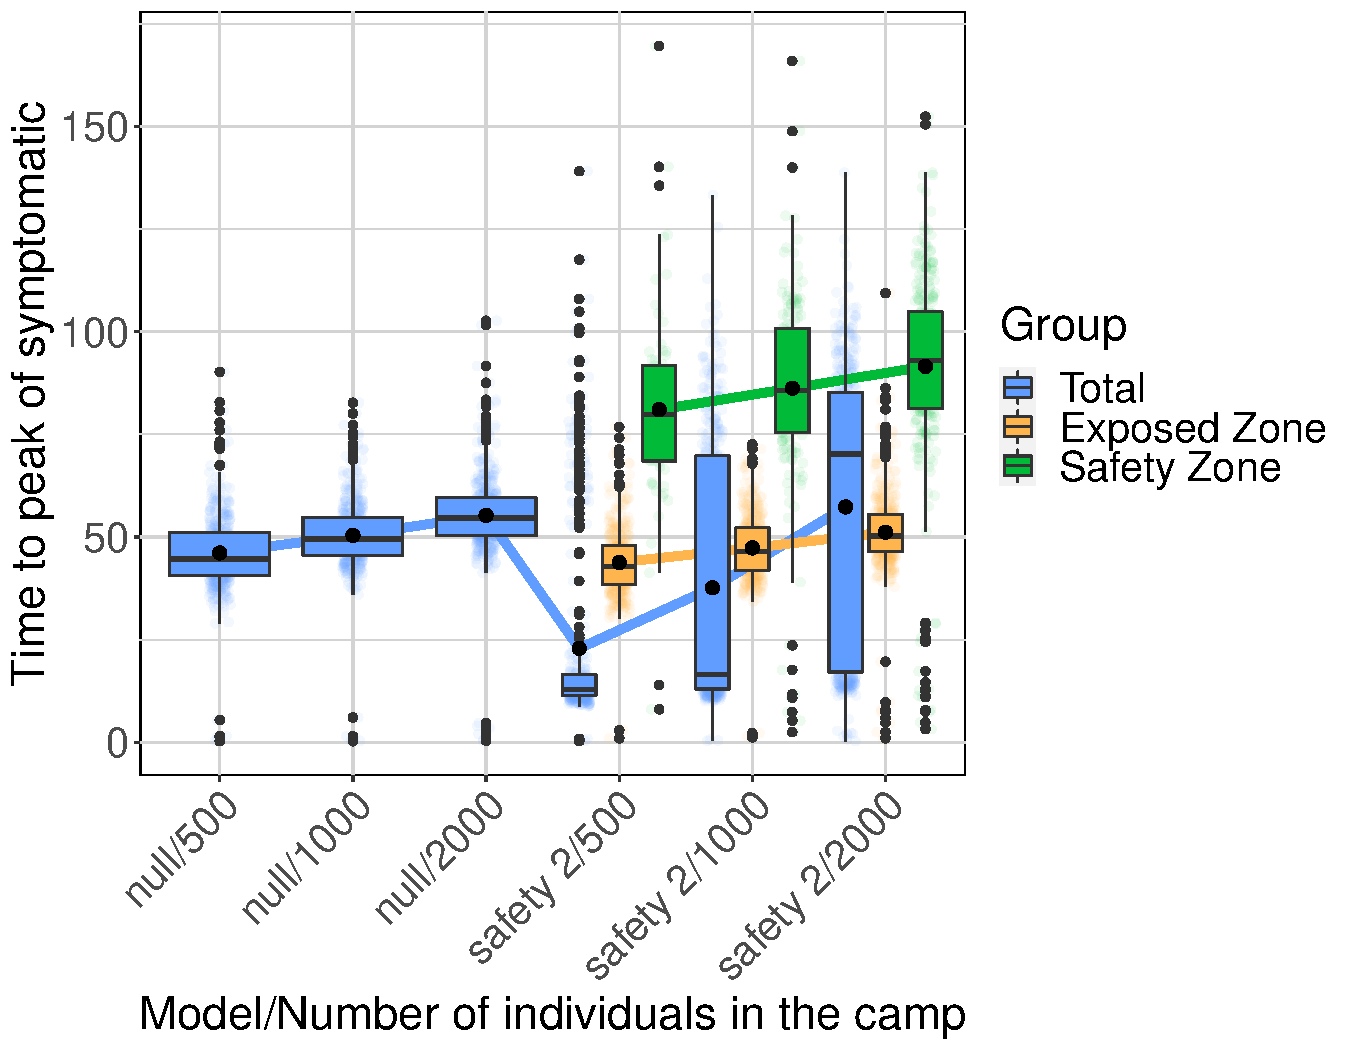
\includegraphics[width=0.31\textwidth]{figures/FigS10c}\\\medskip{}
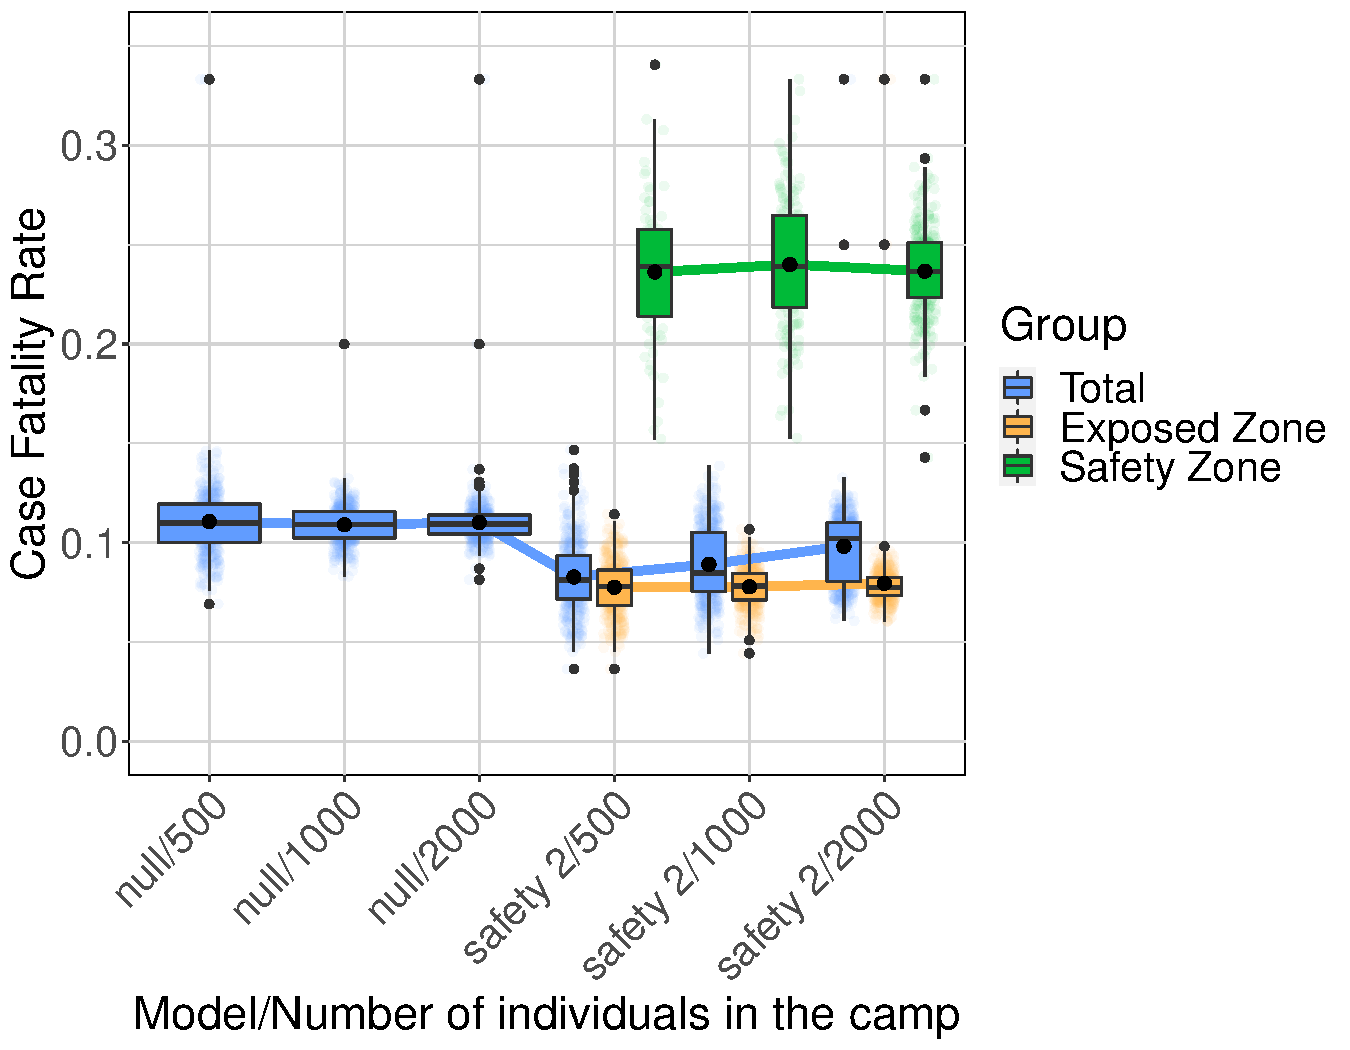
\includegraphics[width=0.31\textwidth]{figures/FigS10d}\hspace{2mm}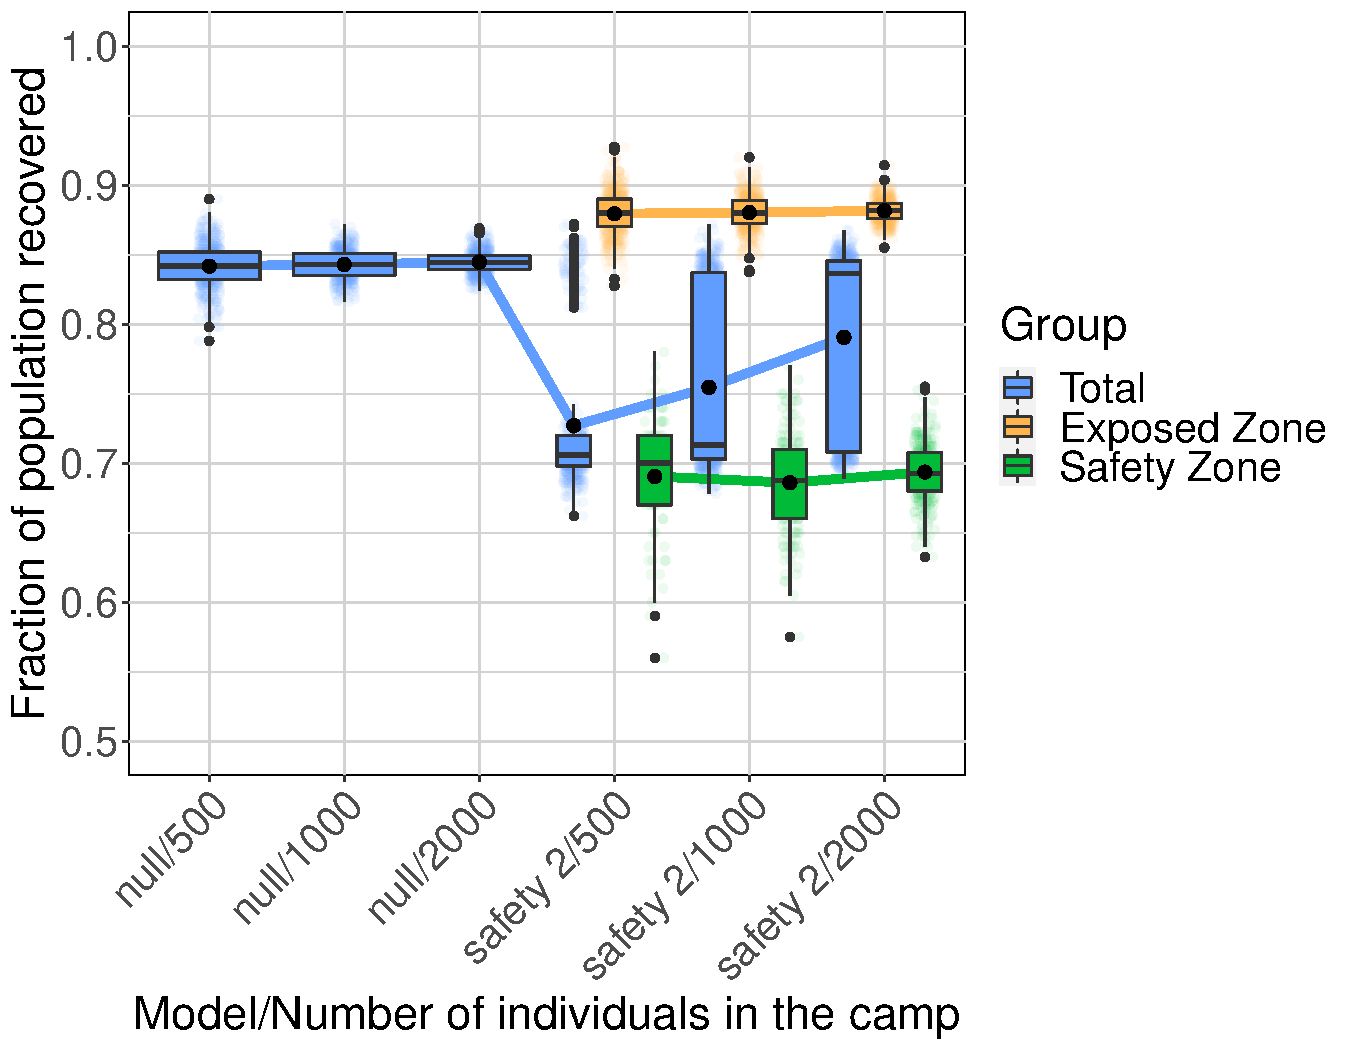
\includegraphics[width=0.31\textwidth]{figures/FigS10e}
\par\end{centering}
\caption{\label{fig:Suppl_popSize} \textbf{Efficiency of safety zone for different
population sizes.} Probability of outbreak (top-left), fraction of
casualties (top-middle), time in which the number of symptomatic cases
peaks (top-right), CFR (bottom-left) and fraction of recovered individuals
(bottom-right), as a function of the total population size of the
camp.}
\end{figure}

\medskip{}

\begin{figure}[H]
\begin{centering}
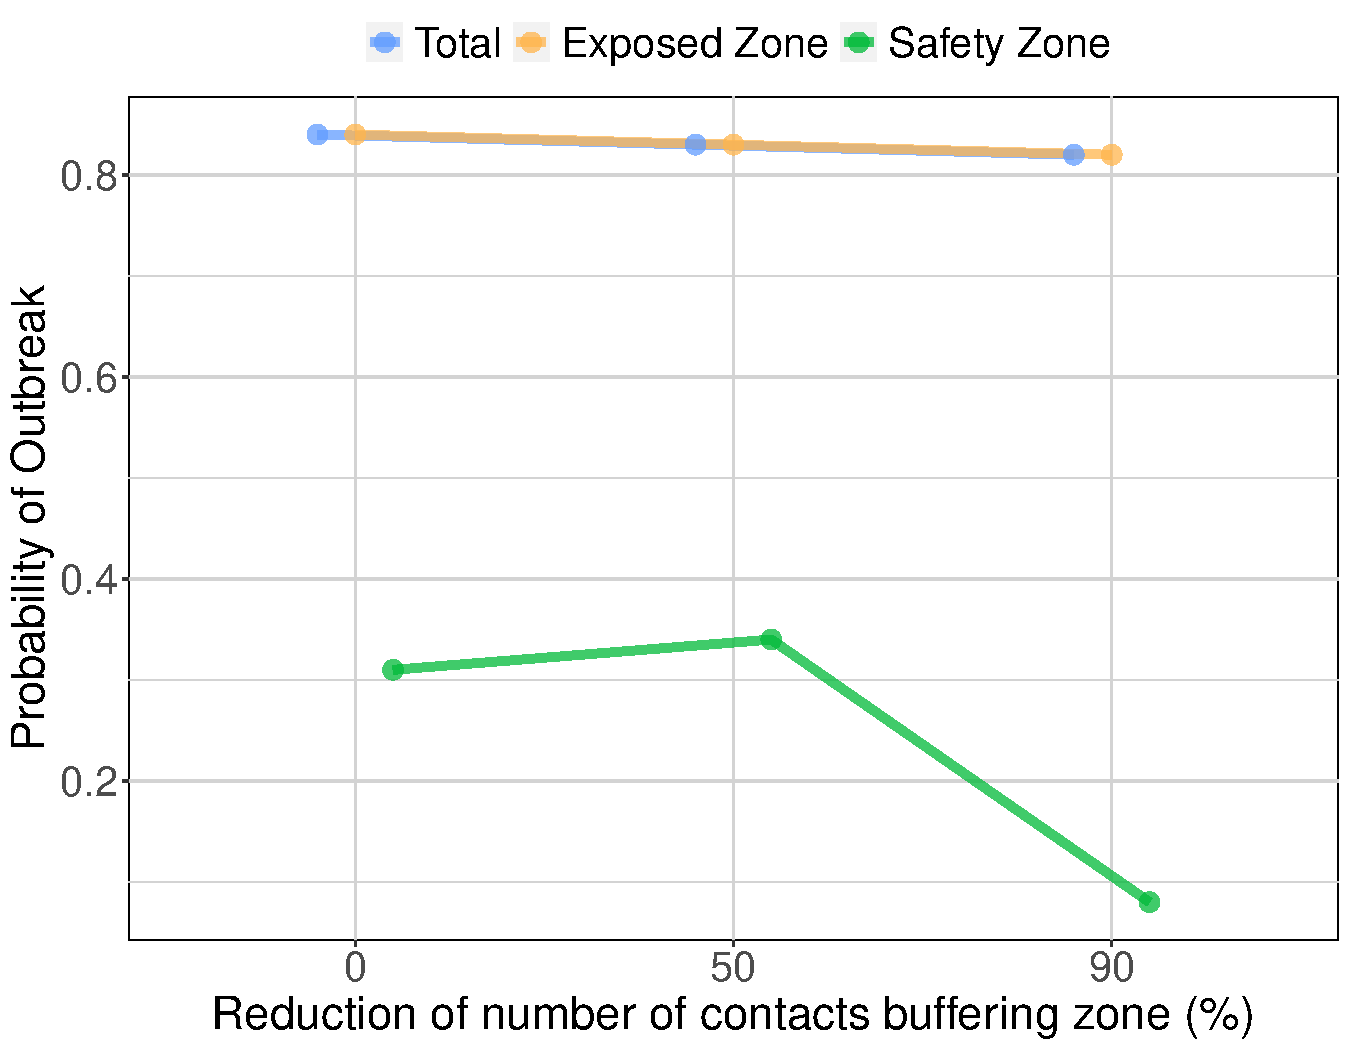
\includegraphics[width=0.31\textwidth]{figures/FigS11a}\hspace{2mm}\includegraphics[width=0.31\textwidth]{figures/FigS11b}\hspace{2mm}\includegraphics[width=0.31\textwidth]{figures/FigS11c}\\\medskip{}
\includegraphics[width=0.31\textwidth]{figures/FigS11d}\hspace{2mm}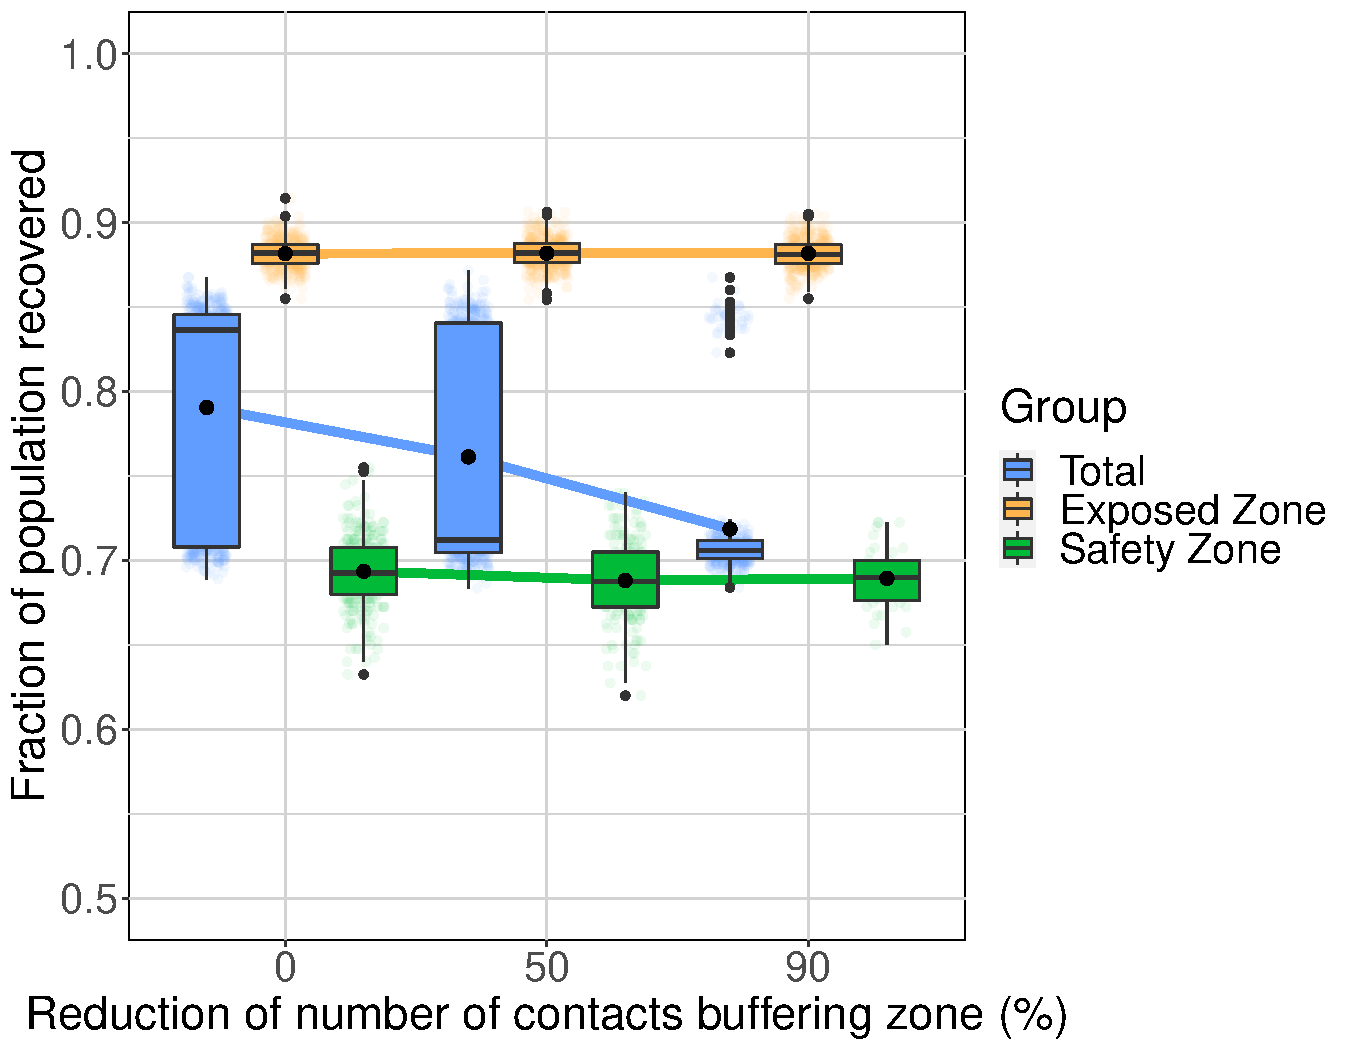
\includegraphics[width=0.31\textwidth]{figures/FigS11e}
\par\end{centering}
\caption{\label{fig:Suppl_popSize-1} \textbf{Lockdown of the safety zone.}
Probability of outbreak (top-left), fraction of casualties (top-middle),
time in which the number of symptomatic cases peaks (top-right), CFR
(bottom-left) and fraction of recovered individuals (bottom-right),
as a function of the reduction in the number of contacts permitted
in the buffering zone.}
\end{figure}

\begin{thebibliography}{1}
\bibitem[1]{key-1}Li, Q., Guan, X., Wu, P., Wang, X., Zhou, L., Tong,
Y., ... \& Xing, X. (2020). Early transmission dynamics in Wuhan,
China, of novel coronavirus--infected pneumonia. New England Journal
of Medicine.

\bibitem[2]{key-2}He, X., Lau, E. H., Wu, P., Deng, X., Wang, J.,
Hao, X., ... \& Mo, X. (2020). Temporal dynamics in viral shedding
and transmissibility of COVID-19. Nature medicine, 26(5), 672-675.

\bibitem[3]{key-3}Wölfel, R., Corman, V. M., Guggemos, W., Seilmaier,
M., Zange, S., Müller, M. A., ... \& Hoelscher, M. (2020). Virological
assessment of hospitalized patients with COVID-2019. Nature, 581(7809),
465-469.

\bibitem[4]{key-4}Wang D, Hu B, Hu C, et al. Clinical Characteristics
of 138 Hospitalized Patients With 2019 Novel Coronavirus--Infected
Pneumonia in Wuhan, China. JAMA. 2020;323(11):1061--1069. doi:10.1001/jama.2020.1585

\bibitem[5]{key-5}McLaws, L. (2020). Estimating the extent of asymptomatic
COVID-19 and its potential for community transmission: systematic
review and meta-analysis (Doctoral dissertation, Bond university).

\bibitem[6]{key-6}Coronavirus Disease 2019 in Children --- United
States, February 12--April 2, 2020. MMWR Morb Mortal Wkly Rep 2020;69:422--426.
DOI: http://dx.doi.org/10.15585/mmwr.mm6914e4external icon

\bibitem[7]{key-7}CDC COVID-19 Response Team. Preliminary Estimates
of the Prevalence of Selected Underlying Health Conditions Among Patients
with Coronavirus Disease 2019 - United States, February 12-March 28,
2020. MMWR Morb Mortal Wkly Rep. 2020;69(13):382-386. Published 2020
Apr 3. doi:10.15585/mmwr.mm6913e2
\end{thebibliography}

\section*{%
\begin{comment}
Leftovers

\textbf{Maximum number of family members permitted}

{[}APG, the following should be reviewed, it is unfinished{]} We considered
until now that people from the orange area visiting the buffering
zone will be always different within the same week. An interesting
question for management is how to keep the fraction of the orange
population using the buffering zone as small as possible to minimize
the spread of the infection. This relies on the assumption that, since
symptomatic members are excluded from the buffering zone, increasing
this fraction increases the chances for assymptomatic or presymptomatic
individuals to visit the buffering zone. As we will see immediately,
this observation could be used to improve the management strategies.

To illustrate this point we note that the fraction of the orange population
getting in contact with the green population can be estimated through
the quantity $0.2\epsilon_{ij}m_{ij}$ ($i\in\oran$), which we aim
to keep lower than one. Expanding this expression we obtain

\[
c_{\family}<5\sqrt{\bar{c}_{i}\frac{N_{\oran}}{N}}
\]

with a value of $\approx17$ individuals per day for the adult class
and assuming 20\% of the population shielded. Note that the estimation
heavily relies on the efficiency of the protection measures.

\textbf{The clan's dilemma}

In the previous section, we considered that the family members visiting
were always different. However, if the population in the camps is
structured in large families (hereafter clans) it opens the question
of whether it would be more beneficial to keep all members of the
same clan in the same area or in different areas. If all members of
the same clan live in the same zone, there would be little need to
interact with members of the other zone, hence reducing $c_{\family}$.
However, since the capacity of the green zone is limited, shielding
whole clans may lead to leaving other clans completely outside of
the green zone, even if the strategy may be better to minimize the
overall impact in the population. On the other hand, if clans are
split, it increases the chances that the same relatives visit the
buffering zone several times. Under the assumption that minimizing
the number of different people would reduce the probability of infection,
this could also be a positive strategy.
\end{comment}
}

\bibliographystyle{plain}
\bibliography{req550-syria}

\end{document}
